\label{ch:advection}


\section{The linear advection equation}

The linear advection equation is simply:
\begin{equation}
\label{eq:advect}
a_t + u a_x = 0
\end{equation}
where $a(x,t)$ is some scalar quantity and $u$ is the velocity at
which it is advected ($u > 0$ advects to the right).  The solution to
Eq.~\ref{eq:advect} is to simply take the initial data, $a(x,t=0)$,
and displace it to the right at a speed $u$.  The shape of the initial
data is preserved in the advection.  Many hyperbolic systems of PDEs,
e.g.\ the equations of hydrodynamics, can be written in a form that
looks like a system of (nonlinear) advection equations, so the
advection equation provides important insight into the methods used
for these systems.
%
\begin{exercise}[Linear advection analytic solution]
{Show via substitution that $a(x - ut)$ is a solution to
  Eq.~\ref{eq:advect} for any choice of a.  This means that
the solution is constant along the lines $x = u t$
(the curves along which the solution is constant are called the
characteristics).}
\end{exercise}

Figure~\ref{fig:advection_char} shows an initial profile, $a(x)$, and
the corresponding characteristics in the $t$-$x$ plane.  With time,
since the solution is constant along these characteristics, it simply
each point simply follows the characteristic curve, resulting in a
shift of the profile to the right.

An important concept that we will discuss shortly is {\em stability}.
Not every discretization that we write down will be well behaved.  For
some, our initial state will begin to ``blow-up'', and take on
obscenely large and unphysical values after just a few steps.  This is
the hallmark of a method that is unstable.  Some methods have
restrictions on the size of the timestep that result in a stable
methods as well.

% this figure is produced by figures/advection/characteristics.py
\begin{figure}[t]
\centering
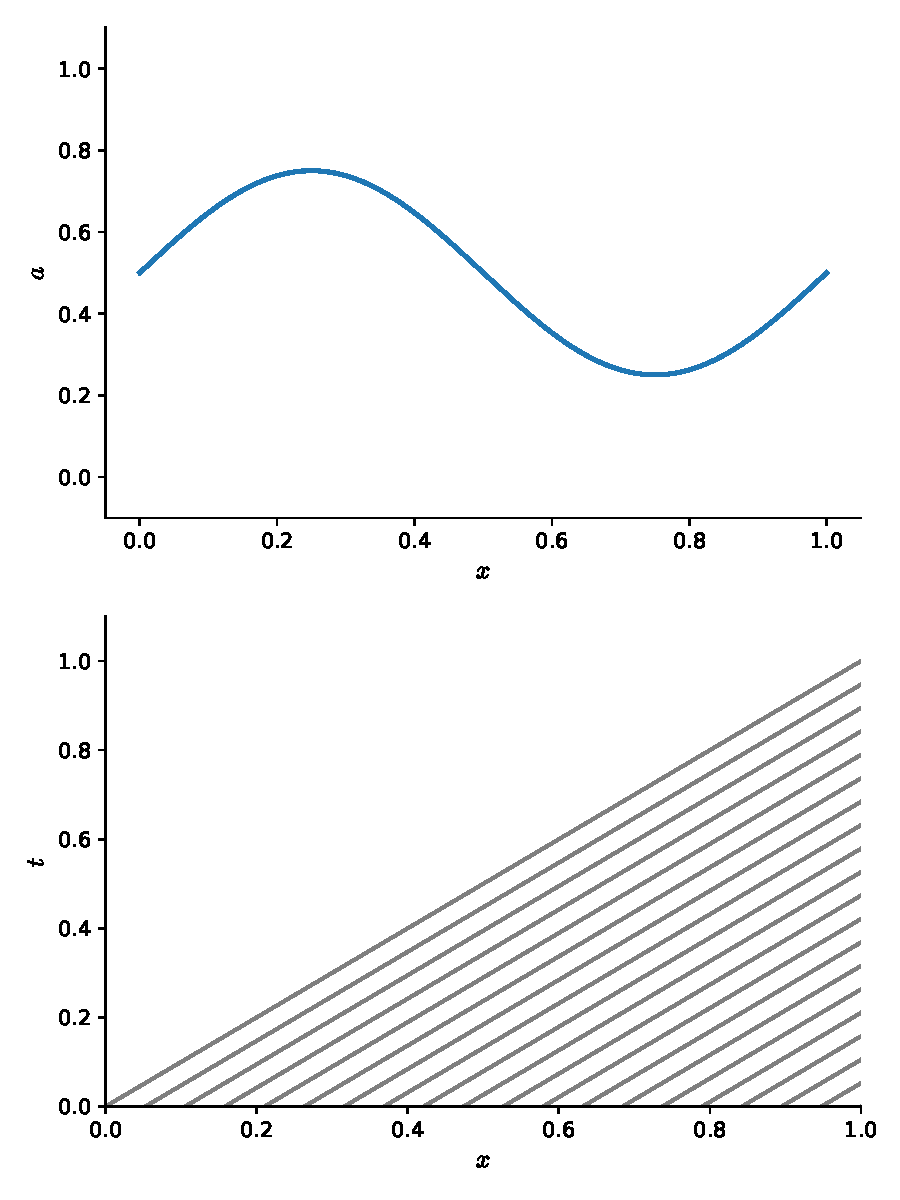
\includegraphics[width=0.6\linewidth]{advection-characteristics}
\caption[Characteristics for linear advection]
{\label{fig:advection_char} (top) Initially sinusoidal
distribution (bottom) Characteristic
structure for the linear advection equation $u = 1$.  Note
that for this linear equation the characteristics are all parallel
(they have the same slope in the $t$-$x$ plane.}
\end{figure}

\section{First-order advection in 1-d and finite-differences}

To get a flavor of the methods for advection, we will use a simple
finite-difference discretization---here, the domain is divided into
a sequence of points where we store the solution.
We will solve
Eq.~\ref{eq:advect} numerically by discretizing the solution at
these points.  The index $i$ denotes the point's location, and $a_i$
denotes the discrete value of $a(x)$ in zone $i$.  The data in each
zone can be initialized as $a_i = a(x_i)$.  Figure~\ref{fig:fdgrid}
shows the grid.

We also need to discretize in time.  We denote the time-level of the
solution with a superscript, so $a_i^n = a(x_i,t^n)$.  For a fixed
$\Delta t$, time level $n$ corresponds to a time of $t = n\Delta t$.


A simple first-order accurate discretization is:
\begin{equation}
\frac{a_i^{n+1} - a_i^n}{\Delta t} = - u \frac{a_i^n - a_{i-1}^n}{\Delta x}
\label{eq:fo}
\end{equation}
This is an {\em explicit} method, since the new solution, $a_i^{n+1}$,
depends only on information at the old time level, $n$.  

Finally, we also need to specify a boundary condition for this.  Our
choice of spatial derivative is one-sided---it uses information from
the zone to the left of the zone we are updating.  This is because
information is flowing from left to right in this problem ($u > 0$).
This choice of the derivative is called {\em upwinding}---this choice
of derivative results in a stable method.
Notice that if we use Eq.~\ref{eq:fo} to update the data in the first
zone inside the boundary, we need data to the left of this
zone---outside of the domain.  This means that we need a single
{\em ghost point} to implement the boundary conditions for our method.  The
presence of the ghost points allow us to use the same update equation
(e.g.\ Eq.~\ref{eq:fo}) for all zones in the domain.


% figure created by figures/advection/fd-ghost.py
\begin{figure}[t]
\centering
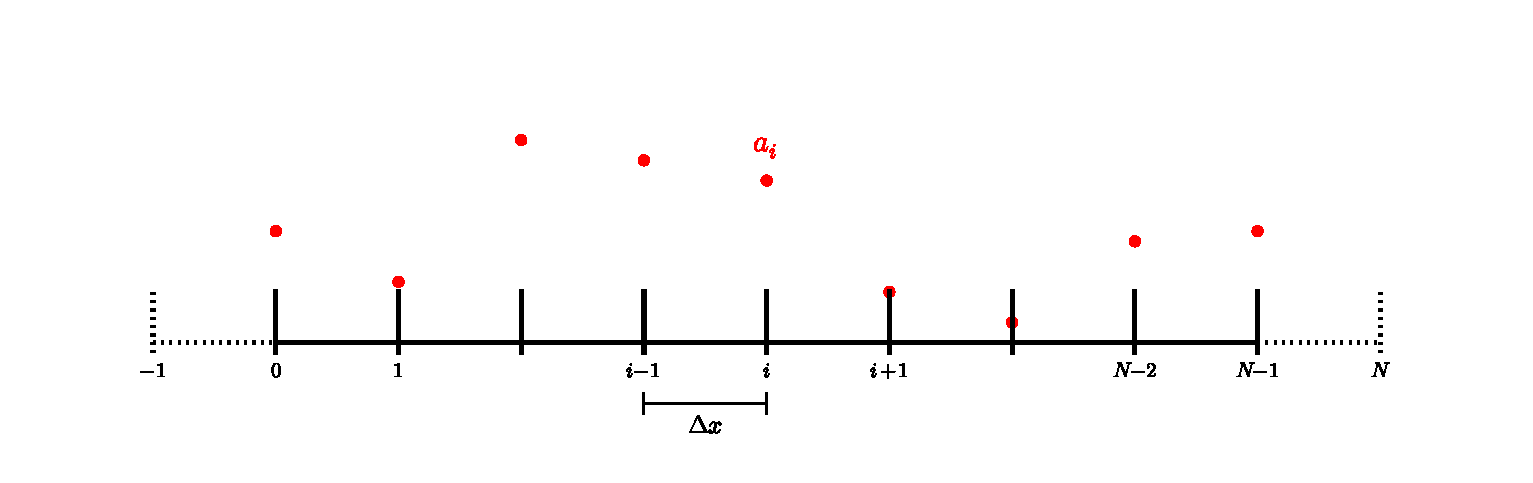
\includegraphics[width=\linewidth]{fd_ghost}
\caption[A simple finite-difference grid]{\label{fig:fdgrid} A simple
  finite-difference grid.  The solution is stored at each of the
  labeled points.  The dotted lines show the ghost points used to
  extend our grid past the physical boundaries to accommodate boundary
  conditions.  Note that if we are periodic, then points $0$ and $N-1$
  are at the same physical point in space, so we would only need to
  update one of them.}
\end{figure}

The last piece of information needed to update the solution is the
timestep, $\Delta t$.  It can be shown that for the solution to be
{\em stable}, the timestep must be less than the time it takes information
to propagate across a single zone.  That is:
\begin{equation}
\Delta t \le \frac{\Delta x}{u} \enskip .
\end{equation}
This is called the {\em Courant-Friedrichs-Lewy} or {\em CFL}
condition.  A dimensionless quantity called the {\em CFL number} is 
defined as 
\begin{equation}
\cfl = \frac{\Delta t u }{\Delta x} 
\end{equation}
Stability requires $\cfl \le 1$.
%
We traditionally write the timestep as
\begin{equation}
\label{eq:timestep}
\Delta t = \cfl \frac{\Delta x}{u}
\end{equation}
and specify $\cfl$ as part of the problem (a typical value may be $\cfl = 0.7$).

\begin{exercise}[Perfect advection with a Courant number of 1]
{Show analytically that when you use $\cfl=1$ in the
  first-order differenced advection equation (Eq.~\ref{eq:fo}) that
  you advect the profile exactly, without any numerical error.}
\end{exercise}

Keep in mind that, in general, we will be solving a non-linear
system of equations, so it is not possible to run with $\cfl=1$, 
since $u$ (and therefore $\cfl$) will change from zone to zone.
Instead, one looks at the most restrictive timestep over all the
zones and uses that for the entire system.


\begin{exercise}[A 1-d finite-difference solver for linear advection]
{Write a code to solve the 1-d linear advection equation
  using the discretization of Eq.~\ref{eq:fo} on the domain $[0,1]$ with
  $u=1$ and periodic boundary conditions.  For initial conditions,
  try both a Gaussian profile and a top-hat:}
  \begin{equation}
  a = \left \{
      \begin{array}{lllll}0 & \mathit{~if~~} &         &x& < 1/3 \\
                          1 & \mathit{~if~~} & 1/3 \le &x& < 2/3 \\
                          0 & \mathit{~if~~} & 2/3 \le &x&
      \end{array}
      \right .
  \end{equation}

  \noindent Note: For a general treatment of boundary conditions, you would
    initialize the ghost points to their corresponding periodic data
    and apply the difference equations to zones $0, \ldots, N-1$.
    However, for periodic BCs on this grid, points $0$ and $N-1$ are
    identical, so you could do the update in this special case on
    points $1, \ldots, N-1$ without the need for ghost points and then
    set $a_0 = a_{N-1}$ after the update. \\

  \noindent Run you program for one or more periods (one period
    is $T=1/u$) with several different CFL numbers and notice that
    there is substantial numerical dissipation (see Figure~\ref{fig:fdadvect}).
\end{exercise}

\begin{figure}[t]
\centering
% figure generated by hydro_examples/advection/fdadvect.py
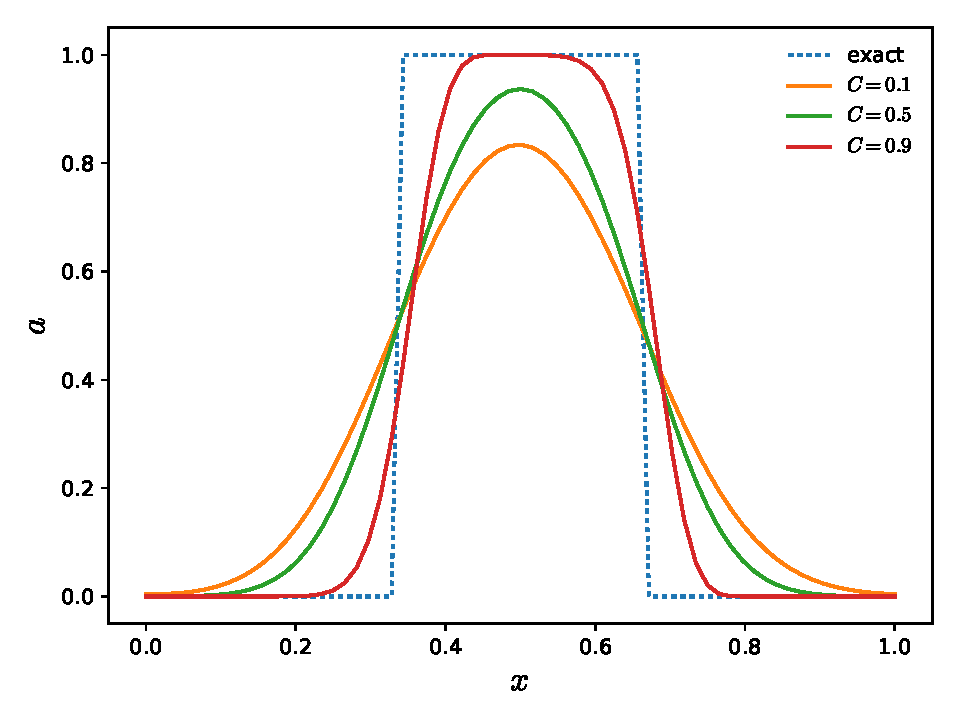
\includegraphics[width=0.8\linewidth]{fdadvect-upwind}
\caption[First-order finite-difference solution to linear advection]
{\label{fig:fdadvect} Finite-difference solution to the first-order
finite-difference upwind method for advection, using 65 points and
a variety of CFL numbers. \\
\hydroexdoit{\href{https://github.com/zingale/hydro_examples/blob/master/advection/fdadvect.py}{fdadvect.py}}}
\end{figure}
%
This method is first-order accurate.  


Ultimately we will want higher-order accurate methods.  The most obvious
change from our initial discretization is to try a higher-order spatial
derivative.

\begin{exercise}[FTCS and stability]
{You may think that using a centered-difference for
  the spatial derivative, $a_x \sim (a_{i+1} - a_{i-1})/(2 \Delta x)$
  would be more accurate.  This method is called FTCS (forward-time,
  centered-space).  Try this on the same test problems.}
\end{exercise}

\begin{figure}[t]
\centering
% figure generated by hydro_examples/advection/fdadvect.py
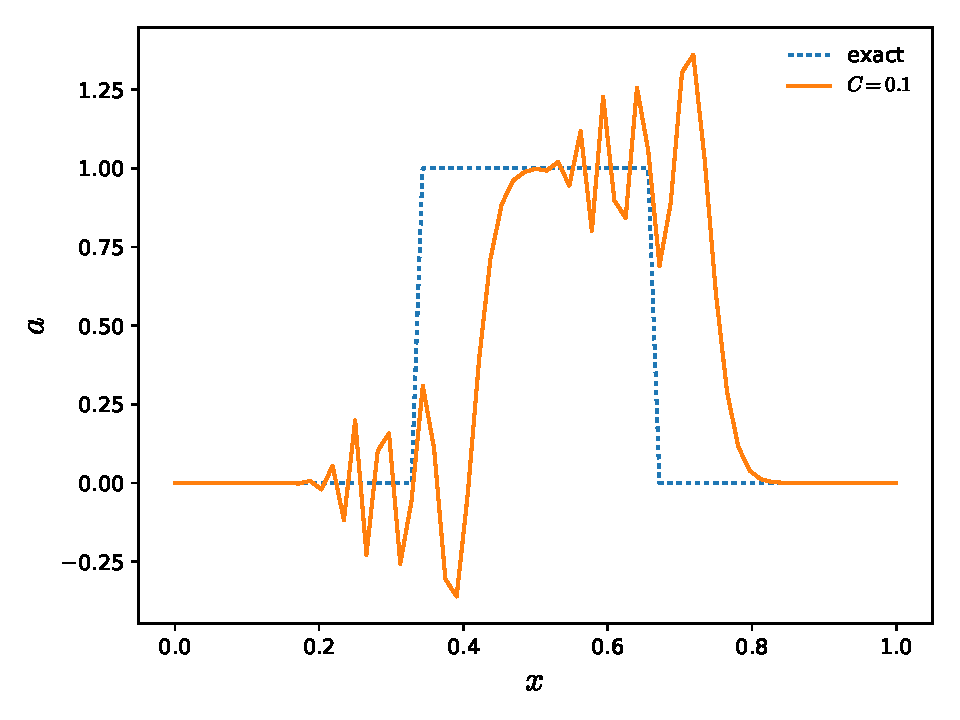
\includegraphics[width=0.48\linewidth]{fdadvect-FTCS-C0_1}
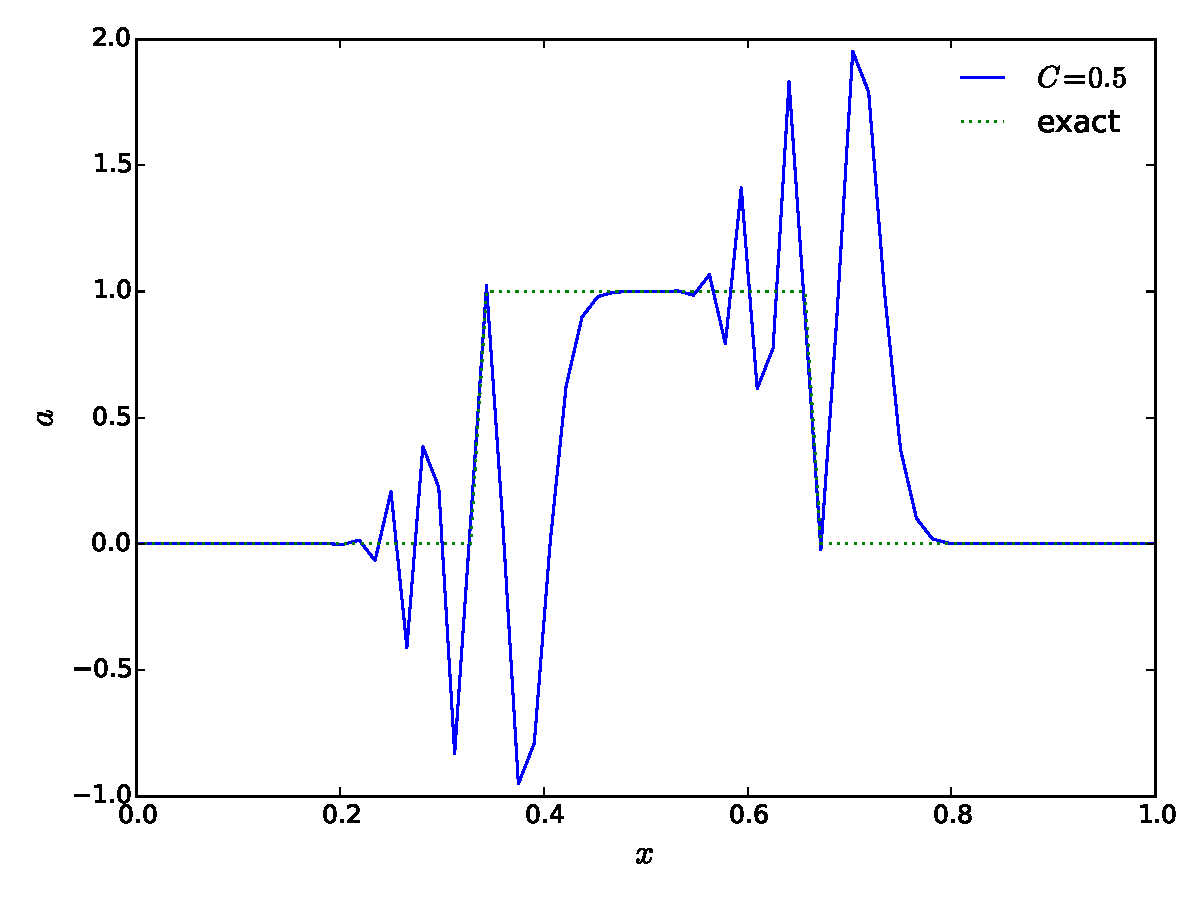
\includegraphics[width=0.48\linewidth]{fdadvect-FTCS-C0_5}
\caption[FTCS finite-difference solution to linear advection]
{\label{fig:fdadvect-ftcs} Finite-difference solution using the FTCS
finite-difference method for advection using 65 points, modeling for
only 1/10$^\mathrm{th}$ of a period.  The panel of the left is
with $\cfl = 0.1$ and the panel on the right is $\cfl = 0.5$.\\
\hydroexdoit{\href{https://github.com/zingale/hydro_examples/blob/master/advection/fdadvect.py}{fdadvect.py}}}
\end{figure}

You will find that no matter what value of $\cfl$ you choose with the
FTCS method, the solution is unconditionally {\em unstable} (see
Figure~\ref{fig:fdadvect-ftcs}).  If you continue to evolve the
equation with this method, you would find that the amplitude grows
without bound.  There is something about that discretization that
simply gets the physics wrong.


\subsection{Stability}

\MarginPar{add a discussion of domain of dependence}

The classic method for understanding stability is to consider the growth 
of a single Fourier mode in our discretization.  That is, substitute in
$a_i^n = A^n e^{Ii\theta}$, where $I = \sqrt{-1}$\footnote{our use of $i$ and $j$ as spatial indices presents an unfortunate clash of notation here, hence the use of $I$ for the imaginary unit}, and $\theta$ represents a
phase.  A method is stable if $|A^{n+1}/A^n| \le 1$.  FTCS appears as:
\begin{equation}
  a_i^{n +1} = a_i^n - \frac{\cfl}{2} (a_{i+1}^n - a_{i-1}^n)
\end{equation}
Examining a Fourier mode shows that:
\begin{align}
  A^{n+1}e^{Ii\theta} &= A^n e^{Ii\theta} - \frac{\cfl}{2} \left (
      A^n e^{I(i+1)\theta} - A^n e^{I(i-1)\theta} \right ) \\
  A^{n+1} &= A^n  - \frac{\cfl}{2} A^n \left ( e^{I\theta} - e^{-I\theta}\right ) \\
  A^{n+1} &= A^n \left ( 1 - I \cfl \sin\theta \right )
\end{align}
so the magnitude of the amplification is
\begin{equation}
 \left | \frac{A^{n+1}}{A^n}\right |^2 = 1 + \cfl^2\sin^2\theta
\end{equation}
We see that there is no value of $\cfl$ that can make the method stable
($|A^{n+1}/A^n| > 1$ always).  Doing the same analysis for
Eq.~\ref{eq:fo} would show that the upwind method is stable for $0\le
\cfl \le 1$. 

\begin{exercise}[Stability of the upwind method]
{Using the above stability analysis, considering the amplitude of a
  single Fourier mode, show that the growth of a mode for the upwind
  method (Eq.~\ref{eq:fo}) is:
  \begin{equation}
    \left | \frac{A^{n+1}}{A^n} \right |^2 = 
           1 - 2\cfl(1-\cfl)(1-\cos\theta)
  \end{equation}
  and stability requires $2\cfl(1-\cfl) \ge 0$ or $0 \le \cfl \le 1$.
}
\end{exercise}

It is important to note that this stability analysis only works for
linear equations, where the different Fourier modes are decoupled,
nevertheless, we use its ideas for nonlinear advection problems as
well.

Truncation analysis can also help us understand stability.  The idea
here is to keep the higher order terms in the Taylor series to understand
how they modify the actual equation you are trying to solve.

\begin{exercise}[Stability analysis]
{To get an alternate feel for stability, we can ask
  what the terms left out by truncation look like.  That is, we can
  begin with the discretized equation:
\begin{equation}
  a_i^{n+1} - a_i^n = -\frac{u \Delta t}{\Delta x} ( a_i^n - a_{i-1}^n )
\end{equation}
and replace $a_i^{n+1}$ with a Taylor expansion in time, and replace
$a_{i-1}^n$ with a Taylor expansion in space, keeping terms to
$O(\Delta t^3)$ and $O(\Delta x^3)$.  Replacing $\partial a/\partial t$
with $-u \partial a/ \partial x$ in the higher-order terms, show 
that our difference equation more closely corresponds to 
\begin{eqnarray}
\label{eq:advect_trunc_analysis}
a_t + u a_x &=& \frac{u \Delta x}{2} \left ( 1 - \frac{\Delta t u}{\Delta x} \right ) \frac{\partial^2 a}{\partial x^2} \\
            &=& \frac{u \Delta x}{2} (1 - \cfl) \frac{\partial^2 a}{\partial x^2}
\end{eqnarray}
}
\end{exercise}


Notice that the righthand side of Eq.~\ref{eq:advect_trunc_analysis}
looks like a diffusion term, however, if $\cfl > 1$, then the coefficient
of the diffusion is negative---this is unphysical.  This means that
the diffusion would act to take smooth features and make them more
strongly peaked---the opposite of physical diffusion.

For FTCS, a similar truncation analysis would show that the diffusion term
is always negative.

\subsection{Implicit-in-time}

An alternate approach to time-discretization is to do an implicit
discretization.  Here our upwind method would appear as:
\begin{equation}
\frac{a^{n+1}_i - a^n_i}{\Delta t} = -u \frac{a^{n+1}_i - a^{n+1}_{i-1}}{\Delta x}
\end{equation}
We can write this as a linear system with coupled equations:
\begin{equation}
-\cfl a^{n+1}_{i-1} + (1 + \cfl) a^{n+1}_i = a_i^n
\end{equation}
The only change here is that the righthand side is evaluated at the new timelevel,
$n+1$.

If we use periodic boundary conditions, then point $0$ and $N-1$ are
identical, so we only need to update one of these.  Taking $u_0^{n+1} = u_{N-1}^{n+1}$, our system in matrix form appears as:
\begin{equation}
\renewcommand{\arraystretch}{1.5}
\left ( \begin{array}{ccccccc} 
1+\cfl & & & & & & -\cfl \\
-\cfl  & 1+\cfl &  \\
 &  -\cfl & 1+\cfl &  \\
 & & -\cfl & 1+\cfl &  \\
&&&\ddots&\ddots &\\
&&&&-\cfl & 1+\cfl & \\
&&&&& -\cfl &1+\cfl
\end{array}
\right )
%
\left ( \begin{array}{c}
u_1^{n+1} \\
u_2^{n+1} \\
u_3^{n+1} \\
u_4^{n+1} \\
\vdots \\
u_{N-2}^{n+1} \\
u_{N-1}^{n+1} 
\end{array}
\right )
=
\left ( \begin{array}{c}
u_1^{n} \\
u_2^{n} \\
u_3^{n} \\
u_4^{n} \\
\vdots \\
u_{N-2}^{n} \\
u_{N-1}^{n} 
\end{array}
\right )
\end{equation}
This requires a matrix solve---this makes implicit methods generally more
expensive than explicit methods.  However, stability analysis would show
that this implicit discretization is stable for any choice of $\cfl$. (But
one must not confuse stability with accuracy---the most accurate solutions
with this method will still have a small $\cfl$).  Also note that the form of 
the matrix will change depending on the choice of boundary conditions.
Figure~\ref{fig:fdadvect-implicit} shows the result of solving this
implicit system.

\begin{figure}[t]
\centering
% figure generated by hydro_examples/advection/fdadvect_implicit.py
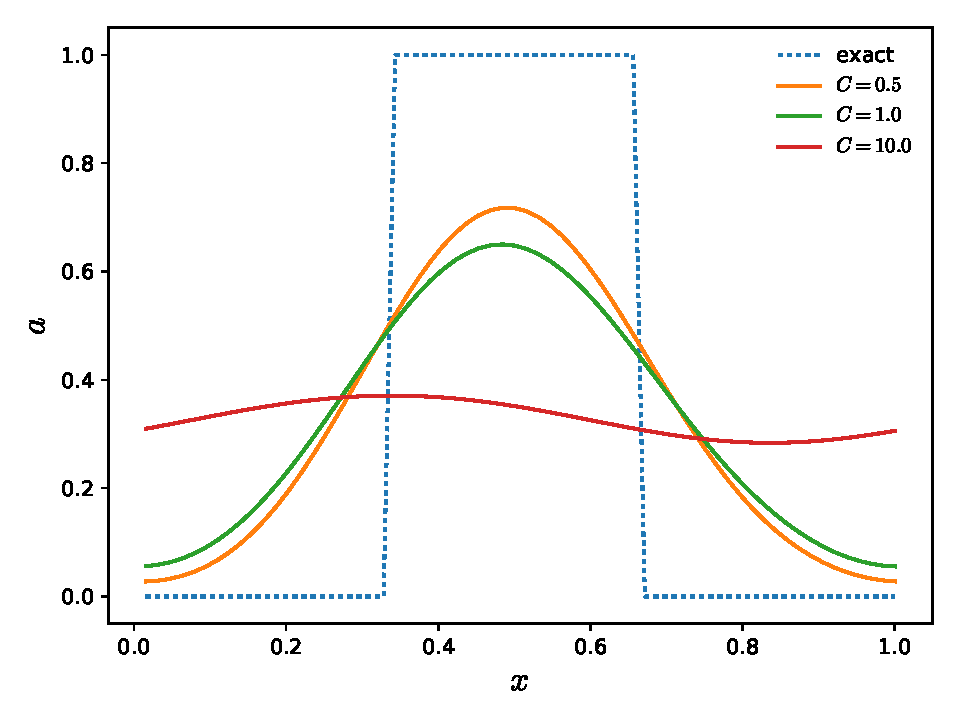
\includegraphics[width=0.8\linewidth]{fdadvect-implicit}
\caption[First-order implicit finite-difference solution to linear advection]
{\label{fig:fdadvect-implicit} Finite-difference solution to the implicit first-order
finite-difference upwind method for advection, using 65 points and
a variety of CFL numbers. \\
\hydroexdoit{\href{https://github.com/zingale/hydro_examples/blob/master/advection/fdadvect_implicit.py}{fdadvect\_implicit.py}}}
\end{figure}

\begin{exercise}[Implicit advection]
{Code up the implicit advection scheme, but using outflow instead of
periodic boundary conditions.  This will change the form of the
matrix.  You can use the code from Figure~\ref{fig:fdadvect-implicit}
as a starting point.}
\end{exercise}


%%%%%%%%%%%%%%%%%%%%%%%%%%%%%%%%%%%%%%%%%%%%%%%%%%%%%%%%%%%%%%%%%%%%%%%%%%%%%%
\section{Eulerian vs.\ Lagrangian frames}

It is useful to think about how our advected quantity, $a(x,t)$, changes in
time.  The full time derivative is:
\begin{equation}
\frac{d a(x,t)}{dt} = \frac{\partial a}{\partial t} + \frac{\partial a}{\partial x}
   \frac{dx}{dt}
\end{equation}
So the value of this derivative depends on the path, $x(t)$, that we choose
to follow.  

Consider an observer who is stationary.  They will watch the flow move
past them, so $dx/dt = 0$, and $da/dt = \partial a/\partial t$.  
This fixed frame is called {\em Eulerian frame}.

Instead imagine an observer who moves with the flow, at the velocity $u$.
This way they keep pace with an individual feature in the flow and track
the changes it experiences.  In this case, $dx/dt = u$, and our derivative,
commonly written as $D/Dt$ is:
\begin{equation}
\frac{D}{Dt} = \frac{\partial}{\partial t} + u \frac{\partial}{\partial x}
\end{equation}
This is the {\em Lagrangian frame}, and the derivative, $D/Dt$ is
called the {\em Lagrangian derivative}, {\em material derivative},
{\em convective derivative}, or {\em advective
derivative}\footnote{and there are actually many more names...}.

Our linear advection equation can be written simply as $Da/Dt = 0$.
We've been solving the equations in the Eulerian frame---our grid is
fixed and the fluid moves through it.  For hydrodynamics, it will be
useful conceptually to consider the Lagrangian frame to understand how
the fluid properties change in a particular fluid element over time.


%%%%%%%%%%%%%%%%%%%%%%%%%%%%%%%%%%%%%%%%%%%%%%%%%%%%%%%%%%%%%%%%%%%%%%%%%%%%%%
\section{Second-order advection in 1-d and the finite-volume method}

\label{ch:adv:sndorder}

In these notes, we will typically use a {\em finite-volume} discretization.  Here we 
explore this method for the 
advection equation.  First we rewrite the advection equation in {\em
  conservation form}:
\begin{equation}
a_t + \left[f(a)\right]_x = 0
\label{eq:advect-cons}
\end{equation}
where $f(a) = ua$ is the flux of the quantity $a$.  In conservation form,
the time derivative of a quantity is related to the divergence of 
its flux.

% figure created with figures/advection/fv-ghost.py
\begin{figure}[t]
\centering
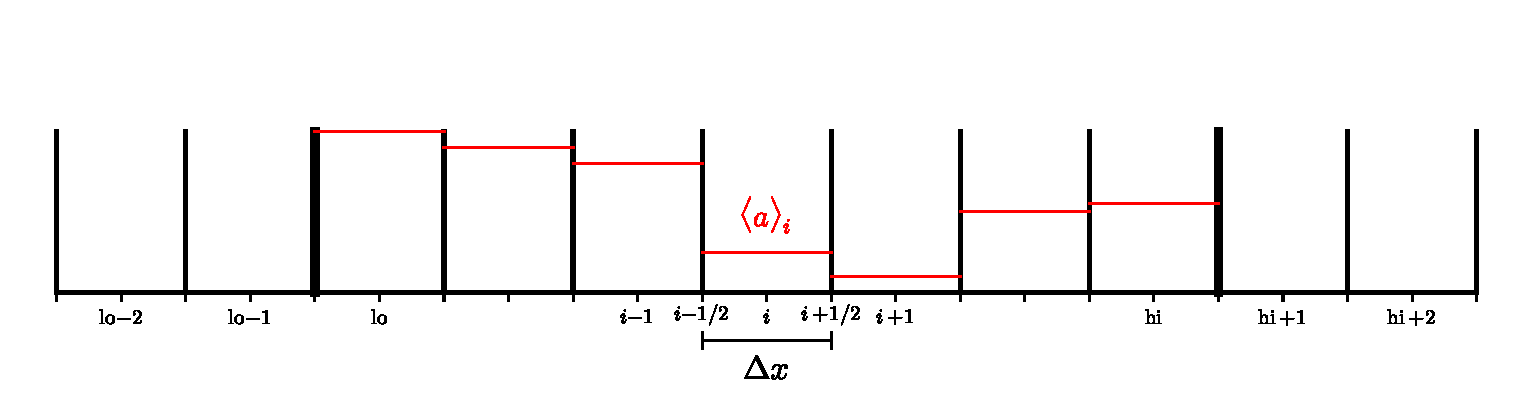
\includegraphics[width=\linewidth]{fv_ghost}
\caption[A finite-volume grid with valid cells
  labeled]{\label{fig:fvghost} A finite-volume grid running from
  $\mathrm{lo}, \ldots, \mathrm{hi}$, with two ghost cells at each
  end.}
\end{figure}

Recall that in the finite-volume discretization, $\langle a\rangle_i$
represents the average of $a(x,t)$ over the interval $x_{i-\myhalf}$ to
$x_{i+\myhalf}$, where the half-integer indexes denote the zone edges
(i.e.\ $x_{i-\myhalf} = x_i - \Delta x/2$).  Figure~\ref{fig:fvghost}
shows an example of such a grid with 2 ghost cells at each end.  (For
simplicity of notation, we drop the $\langle \rangle$ going forward).
To discretize Eq.~\ref{eq:advect-cons}, we integrate it over a zone,
from ${x_{i-\myhalf}}$ to ${x_{i+\myhalf}}$, normalizing by the zone width,
$\Delta x$:
\begin{eqnarray}
\frac{1}{\Delta x} \int_{x_{i-\myhalf}}^{x_{i+\myhalf}} a_t \, dx &=& 
   - \frac{1}{\Delta x} \int_{x_{i-\myhalf}}^{x_{i+\myhalf}} \frac{\partial}{\partial x} f(a) \, dx \\
\frac{\partial}{\partial t} a_i &=& 
   - \frac{1}{\Delta x} \left \{ \left [f(a) \right ]_{i+\myhalf} - \left [f(a) \right ]_{i-\myhalf} \right \}
\end{eqnarray}
This is an evolution equation for the zone-average of $a$, and shows
that it updates in time based on the fluxes through the boundary of
the zone.  We discretize in time by evaluating the righthand side at
the midpoint in time---this gives a centered-difference in time, which
is second-order accurate:
\begin{equation}
\frac{a_i^{n+1} - a_i^n}{\Delta t} = -\frac{\left [f(a) \right ]_{i+\myhalf}^{n+\myhalf} - \left [f(a) \right ]_{i-\myhalf}^{n+\myhalf}}{\Delta x}
\label{eq:consupdate1d}
\end{equation}
To evaluate the fluxes at the half-time, we need the state at the
half-time, that is, we do :
\begin{equation}
\label{adv:eq:fluxeval}
\left [f(a) \right ]_{i+\myhalf}^{n+\myhalf} = f(a_{i+\myhalf}^{n+\myhalf}) \enskip .
\end{equation}
We construct a second-order accurate approximation to
$a_{i+\myhalf}^{n+\myhalf}$ by Taylor expanding the data in the cell to the
interface.  Note that for each interface, there are two possible
interface states we can construct---one using the data to the left of
the interface (which we will denote with a ``L'' subscript) and the
other using the data to the right of the interface (denoted with an
``R'' subscript)---see Figure~\ref{fig:riemann_adv}.  These states are:
\begin{eqnarray}
a_{i+\myhalf,L}^{n+\myhalf} &=& a_i^n + \frac{\Delta x}{2} \left .\frac{\partial a}{\partial x} \right |_i + \frac{\Delta t}{2} \left .\frac{\partial a}{\partial t} \right |_i + \mathcal{O}(\Delta x^2) + \mathcal{O}(\Delta t^2) \nonumber \\
    &=& a_i^n + \frac{\Delta x}{2} \left .\frac{\partial a}{\partial x} \right |_i +  \frac{\Delta t}{2} \left ( - u \left .\frac{\partial a}{\partial x} \right |_i \right ) + \ldots \nonumber \\
    &=& a_i^n + \frac{\Delta x}{2} \left ( 1 - \frac{\Delta t}{\Delta x} u \right ) \left .\frac{\partial a}{\partial x} \right |_i +  \ldots \label{eq:statel}\\
%%
a_{i+\myhalf,R}^{n+\myhalf} &=& a_{i+1}^n - \frac{\Delta x}{2} \left .\frac{\partial a}{\partial x} \right |_{i+1} + \frac{\Delta t}{2} \left .\frac{\partial a}{\partial t} \right |_{i+1} + \mathcal{O}(\Delta x^2) + \mathcal{O}(\Delta t^2) \nonumber \\
    &=& a_{i+1}^n - \frac{\Delta x}{2} \left .\frac{\partial a}{\partial x} \right |_{i+1} +  \frac{\Delta t}{2} \left ( - u \left .\frac{\partial a}{\partial x} \right |_{i+1} \right ) + \ldots \nonumber \\
    &=& a_{i+1}^n - \frac{\Delta x}{2} \left ( 1 + \frac{\Delta t}{\Delta x} u \right ) \left .\frac{\partial a}{\partial x} \right |_{i+1} +  \ldots \label{eq:stater}
\end{eqnarray}
% figure created with figures/advection/riemann.py
\begin{figure}[t]
\centering
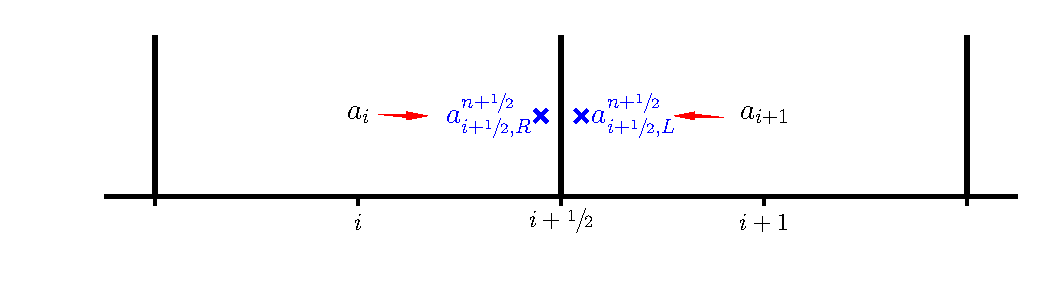
\includegraphics[width=5.0in]{riemann-adv}
\caption[The input state to the Riemann
  problem]{\label{fig:riemann_adv} The left and right interface state
  at the $i+\myhalf$ interface.  Here, the left state,
  $a_{i+\myhalf,L}^{n+\myhalf}$, was predicted to the interface from
  the zone to the left of the interface, using $a_i$, and the right
  state, $a_{i+\myhalf,R}^{n+\myhalf}$, was predicted to the interface
  from the zone to the right, using $a_{i+1}$.}
\end{figure}

A suitable estimate is needed for the slope of $a$ that appears in
these expressions (as $\partial a/\partial x$).  We can approximate
this simply as
\begin{equation}
\left . \frac{\partial a}{\partial x}\right |_i = \frac{a_{i+1} - a_{i-1}}{2 \Delta x} \label{eq:slopecentered}
\end{equation}
We can think of this method as reconstructing the function form of the
data from the cell-average data in each cell using a piecewise linear
polynomial.  Don't be worried that this looks like FTCS---we'll do
upwinding next.


We now have two states, $a_{i+\myhalf,L}^{n+\myhalf}$ and
$a_{i+\myhalf,R}^{n+\myhalf}$ separated by an interface---this is
called the {\em Riemann problem}.
%
The solution to this will depend on the equation being solved, and
results in a single state at the interface:
\begin{equation}
a_{i+\myhalf}^{n+\myhalf} = \mathcal{R}(a_{i+\myhalf,L}^{n+\myhalf},a_{i+\myhalf,R}^{n+\myhalf})
\end{equation}
In our case, the advection equation simply propagates the state to the
right (for $u > 0$), so the solution to the Riemann problem is to take
the left state (this is another example of upwinding).  That is we do:
\begin{equation}
\mathcal{R}(a_{i+\myhalf,L}^{n+\myhalf},a_{i+\myhalf,R}^{n+\myhalf}) = \left \{ \begin{array}{ccc} a_{i+\myhalf,L}^{n+\myhalf} & u > 0 \\[2mm] a_{i+\myhalf,R}^{n+\myhalf} & u < 0 \end{array} \right .
\label{eq:riemannsolve}
\end{equation}
To complete the update, we use this interface state to evaluate the
flux and update the advected quantity via Eq.~\ref{eq:consupdate1d}
and \ref{adv:eq:fluxeval}.

Boundary conditions are implemented by filling the ghost cells outside
each end of the domain based on data in the interior.  Note that at
the very left edge of the domain, the state
$a^{n+\myhalf}_{\mathrm{lo}-\myhalf}$ requires the construction of states on
the left and right.  The left state at that interface,
$a^{n+\myhalf}_{\mathrm{lo}-\myhalf,L}$ depends on the slope reconstructed in
the $\mathrm{lo}-1$ ghost cell, $\partial a/\partial x
|_{\mathrm{lo}-1}$.  This in turn is constructed using a limited
center-difference that will consider the value in the cell to the
left, $\mathrm{lo-2}$.  Therefore, we need two ghost cells at each end
of the domain for this method---figure~\ref{fig:advect_ghost}
illustrates this.  Higher-order limiters may require even more ghost
cells.

% figure from figures/advection/riemann-bc.py
\begin{figure}[t]
\centering
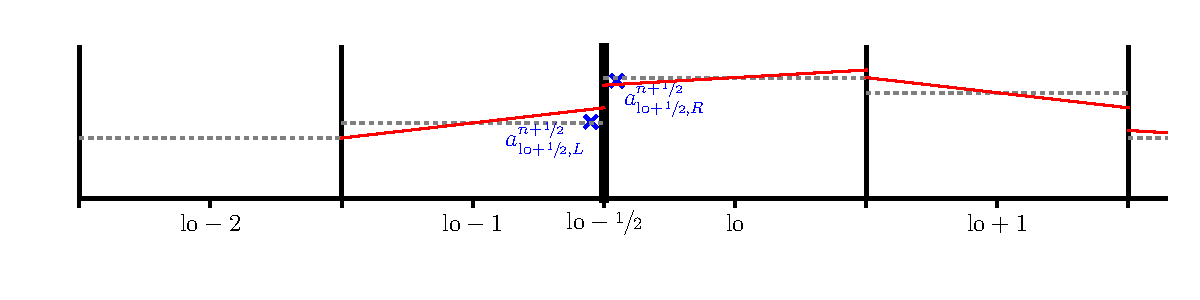
\includegraphics[width=\linewidth]{riemann-bc}
\caption[Reconstruction at the domain boundary]
        {\label{fig:advect_ghost} Reconstruction near the boundary,
          showing the need for two ghostcells.  Here we see the left
          and right state at the left physical boundary of the domain
          (marked as $\mathrm{lo}-\myhalf$).  The gray dotted lines
          are the piecewise constant cell averages and the red lines
          are the reconstructed slopes.  Note that we need the slope
          in $\mathrm{lo}-1$ to get the left interface state at
          $\mathrm{lo}-\myhalf$, and that slope in turn needed the
          data in zone $\mathrm{lo}-2$ to construct a
          centered-difference.}
\end{figure}


\begin{exercise}[A second-order finite-volume solver for linear advection]
{\label{adv:ex:fv} Write a second-order solver for the linear advection
  equation.  To mimic a real hydrodynamics code, your code should have
  routines for finding initializing the state, filling boundary conditions,
  computing the timestep,
  constructing the interface states, solving the Riemann problem, and
  doing the update.  The problem flow should look like:
  \begin{itemize}
    \item set initial conditions
    \item main evolution loop---loop until final time reached
    \begin{itemize}
      \item fill boundary conditions
      \item get timestep (Eq.~\ref{eq:timestep})
      \item compute interface states (Eqs.~\ref{eq:statel} and \ref{eq:stater})
      \item solve Riemann problem at all interfaces (Eq.~\ref{eq:riemannsolve})
      \item do conservative update (Eqs.~\ref{eq:consupdate1d} and \ref{adv:eq:fluxeval})
    \end{itemize}
  \end{itemize}
Use both the top-hat and Gaussian initial conditions and periodic boundary
conditions and compare to the first-order method.  See Figure~\ref{fig:fvadvect}.
}
\end{exercise}

\begin{figure}
\centering
% figure from codes/advection/fv_advection.py
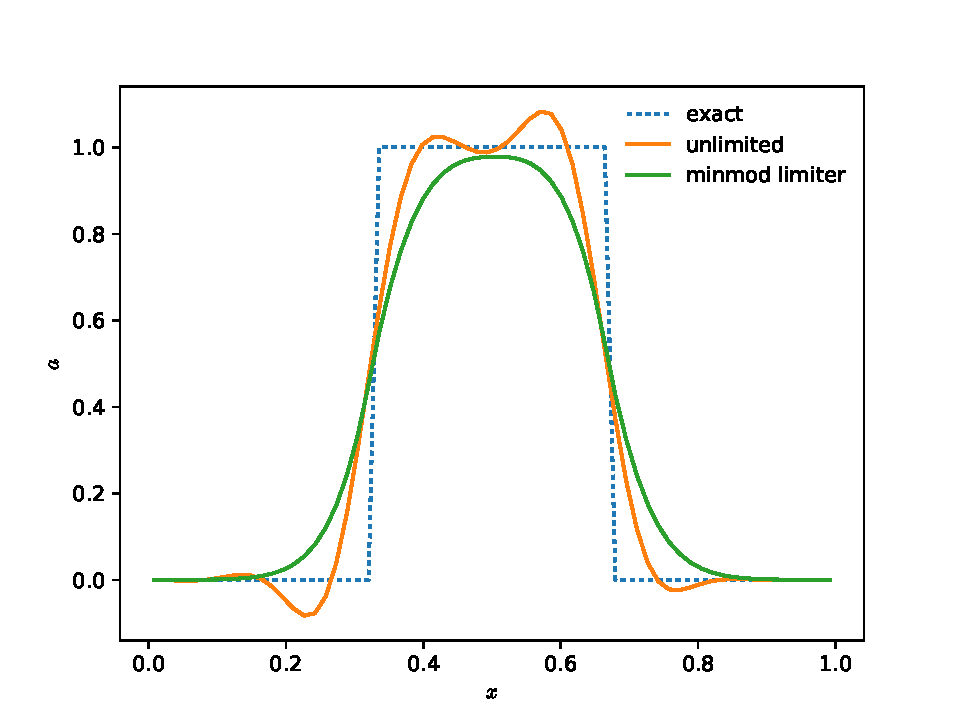
\includegraphics[width=0.8\linewidth]{fv-advect}
\caption[Second-order finite-volume advection]
{\label{fig:fvadvect} Second-order finite volume advection showing the
result of advecting a tophat profile through five periods with both
unlimited and limited slopes.  This calculation used 64 zones and
$\cfl=0.7$. \\ 
\hydroexdoit{\href{https://github.com/zingale/hydro_examples/blob/master/advection/advection.py}{advection.py}}}
\end{figure}

\subsection{Limiting}

The second-order method likely showed some oscillations in the
solution, especially for the top-hat initial conditions.  {\em
  Godunov's theorem} says that any monotonic linear method for
advection is first-order accurate (see, e.g.,~\cite{laney}).  In this
context, monotonic means that no new minima or maxima are introduced.
The converse is true too, which suggests that in order to have a
second-order accurate method for this linear equation, the algorithm
itself must be nonlinear.

\begin{exercise}[Limiting and overshoots]
{To remove the oscillations in
practice, we limit the slopes to ensure that no new minima or maxima are
introduced during the advection process.  There are many choices for
limited slopes.  A popular one is the {\em minmod} limiter.  Here, we
construct the slopes in the interface states as:
\begin{equation}
\left . \frac{\partial a}{\partial x} \right |_i = \mathtt{minmod} \left (
  \frac{a_i - a_{i-1}}{\Delta x}, \frac{a_{i+1} - a_i}{\Delta x} \right )
\end{equation}
instead of Eq.~\ref{eq:slopecentered}.
with 
\begin{equation}
\mathtt{minmod}(a,b) = \left \{ 
    \begin{array}{ll}
    a & \mathit{if~} |a| < |b| \mathrm{~and~} a\cdot b > 0 \\
    b & \mathit{if~} |b| < |a| \mathrm{~and~} a\cdot b > 0 \\
    0 & \mathit{otherwise}
    \end{array}
  \right .
\end{equation}
Use this slope in your second-order advection code and notice that the
oscillations go away---see Figure~\ref{fig:fvadvect}.}
\end{exercise}

We can get a feel for what happens with and without limiting
pictorially. \MarginPar{add a discussion on how a limiter is
  designed/constructed} Figures~\ref{fig:limitingex} and
\ref{fig:limitingexb} show the evolution of an initial discontinuity
with and without limiting.  Without limiting, we see an overshoot
behind the discontinuity and an undershoot ahead of it---these develop
after only a single step.  With each additional step, the overshoots
and undershoots move further away from the discontinuity.  In
contrast, the case with limiting shows no over- or undershoots around
the initial discontinuity.  By the end of the evolution, we see that
the profile is much narrower in the limiting case than in the case
without limiting.

See the text by LeVeque~\cite{leveque:2002} for alternate choices of
limiters. Note: most limiters will have some sort of test on the
product of a left-sided and right-sided difference ($a\cdot b$
above)---this is $< 0$ at an extremum, which is precisely where we
want to limit.

% these two sets of figures can be created with
% figures/advection/rea-limitex.py
\begin{figure}[h]
\centering
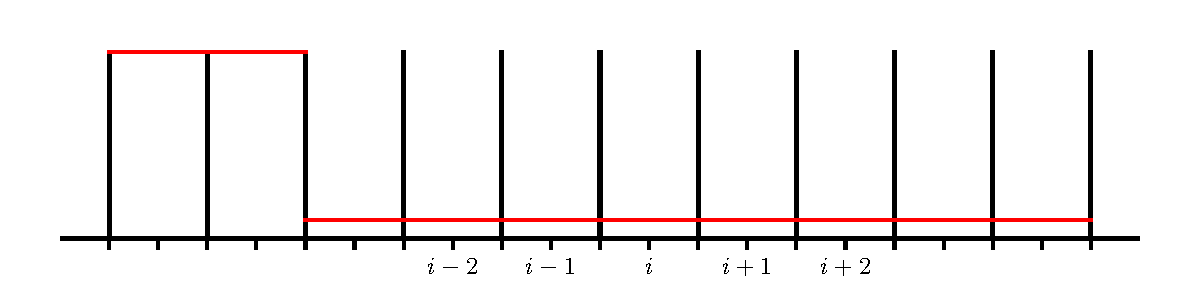
\includegraphics[width=0.75\linewidth]{rea-nolimit-start_001} \\
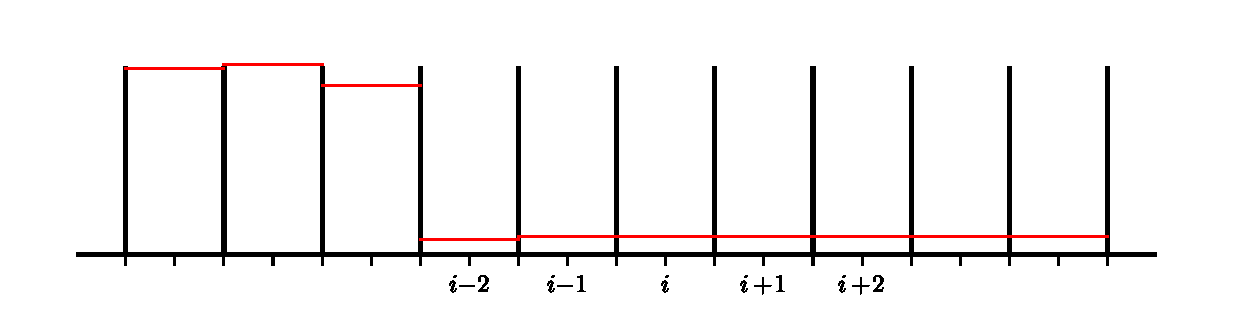
\includegraphics[width=0.75\linewidth]{rea-nolimit-start_002} \\
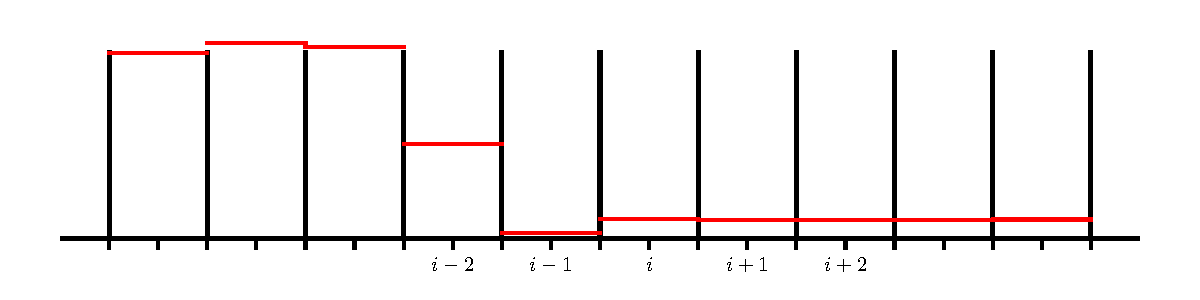
\includegraphics[width=0.75\linewidth]{rea-nolimit-start_003} \\
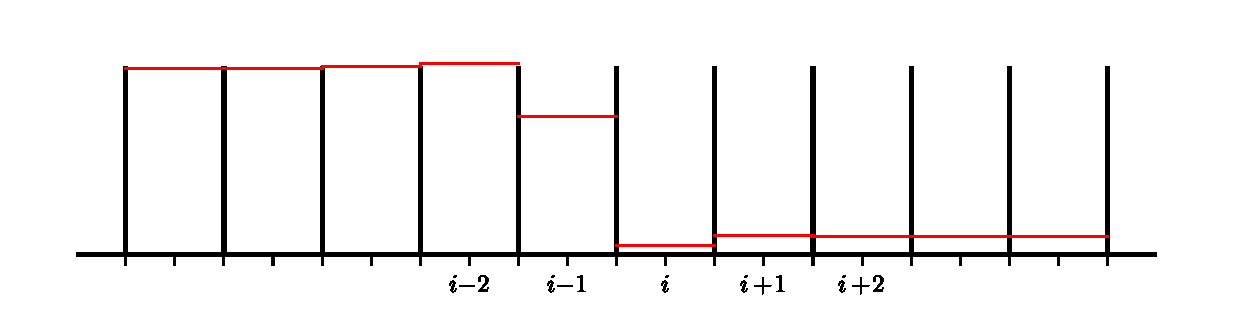
\includegraphics[width=0.75\linewidth]{rea-nolimit-start_004} \\
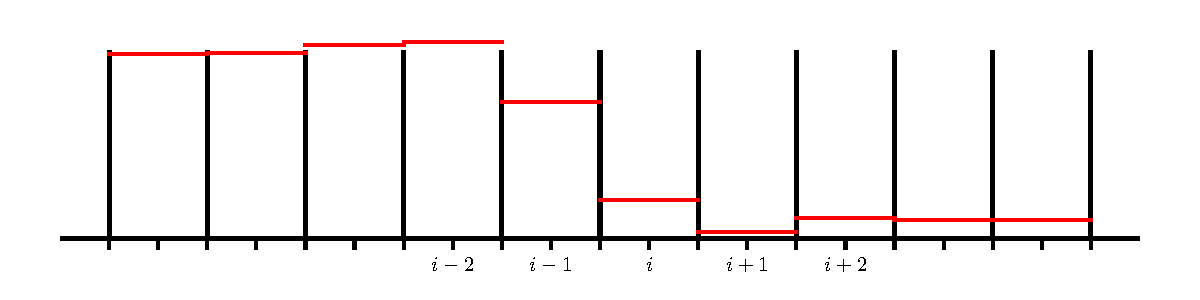
\includegraphics[width=0.75\linewidth]{rea-nolimit-start_005} \\
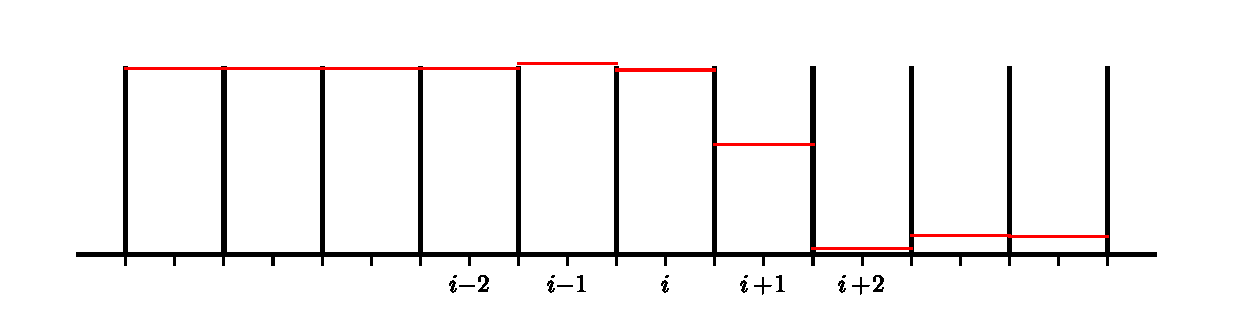
\includegraphics[width=0.75\linewidth]{rea-nolimit-start_006} 
%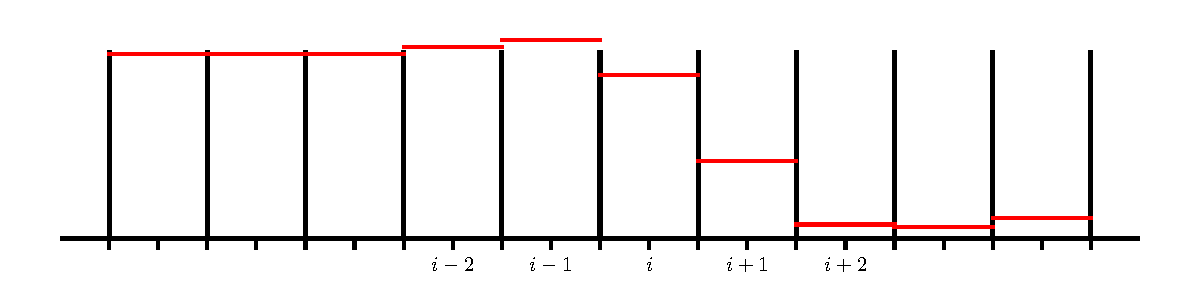
\includegraphics[width=0.55\linewidth]{rea-nolimit-start_007} \\
%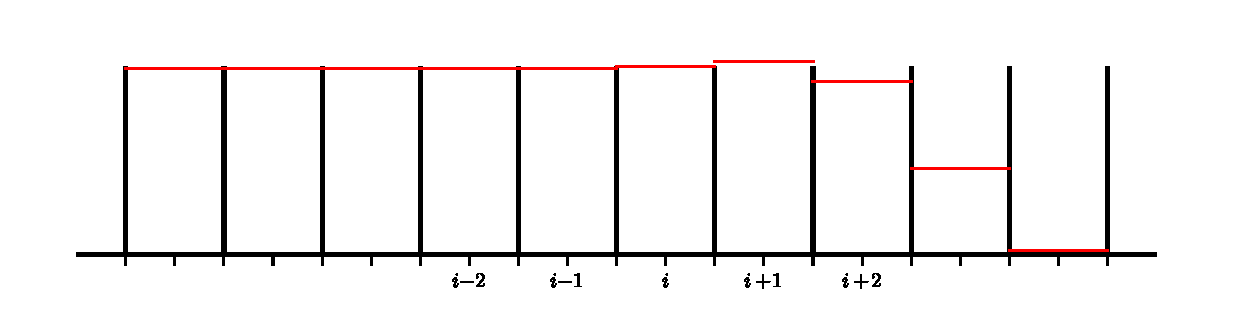
\includegraphics[width=0.55\linewidth]{rea-nolimit-start_008} \\
\caption[The effect of no limiting on initially discontinuous data]{\label{fig:limitingex}Initially discontinuous data evolved for several steps with
  no limiting.  Notice that there are overshoots and undershoots
  surrounding the discontinuity.}
\end{figure}

\begin{figure}[h]
\centering
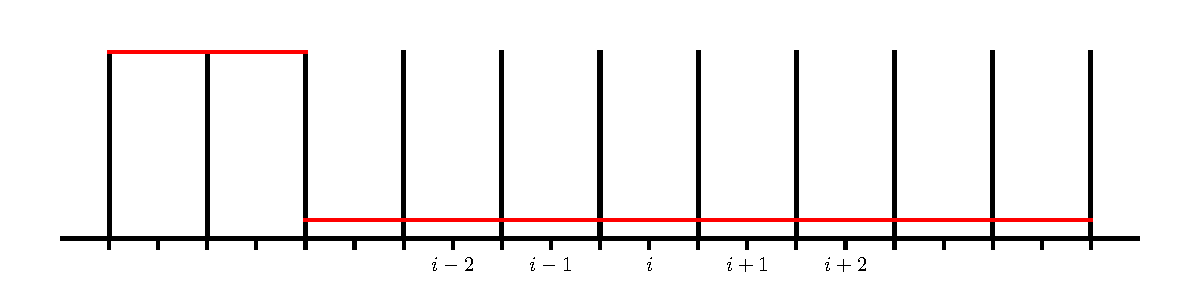
\includegraphics[width=0.75\linewidth]{rea-start_001} \\
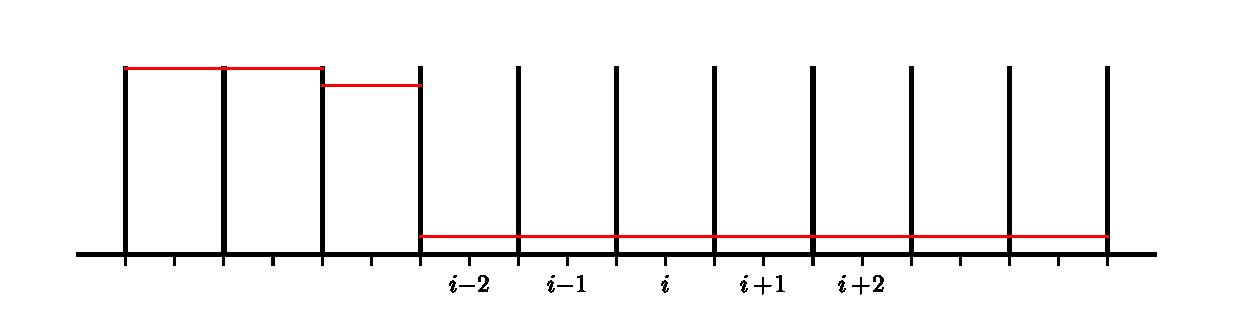
\includegraphics[width=0.75\linewidth]{rea-start_002} \\
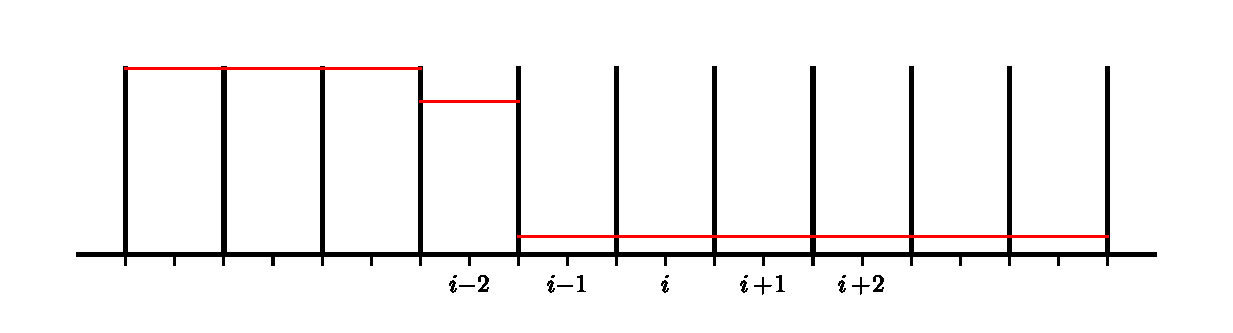
\includegraphics[width=0.75\linewidth]{rea-start_003} \\
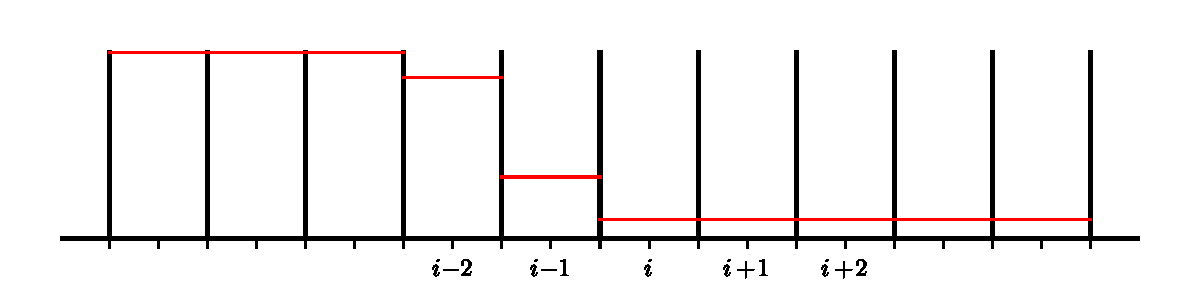
\includegraphics[width=0.75\linewidth]{rea-start_004} \\
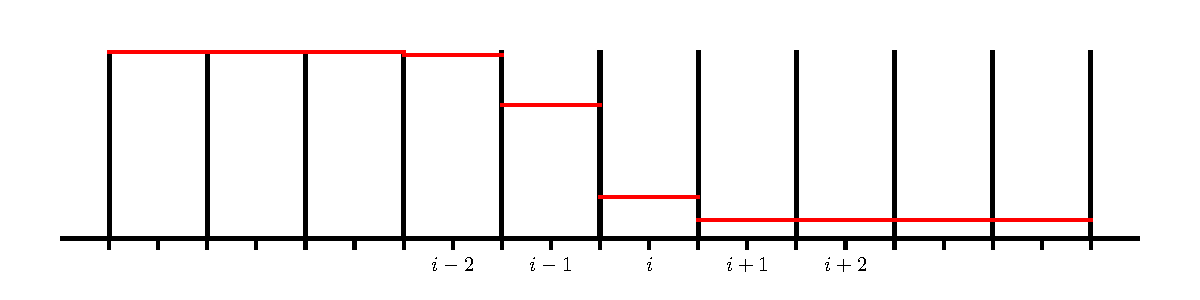
\includegraphics[width=0.75\linewidth]{rea-start_005} \\
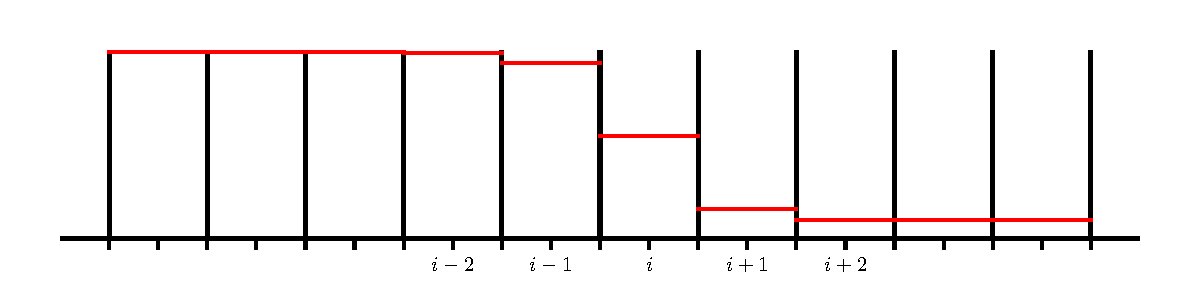
\includegraphics[width=0.75\linewidth]{rea-start_006}
%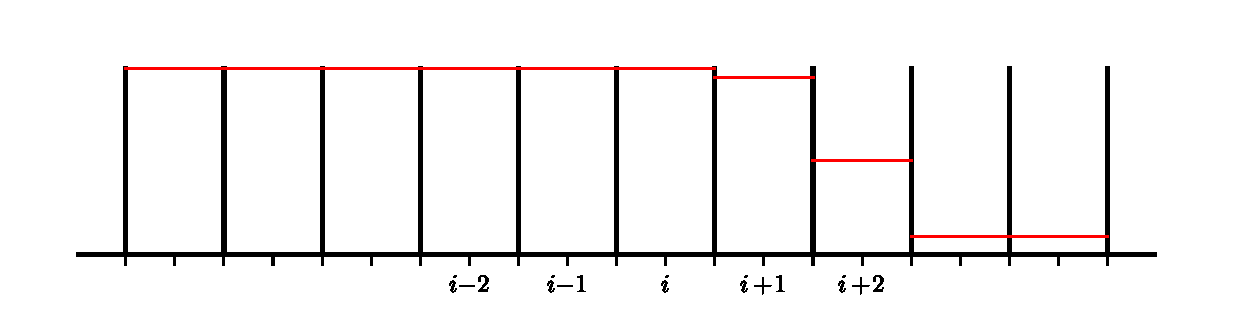
\includegraphics[width=0.55\linewidth]{rea-start_007}
%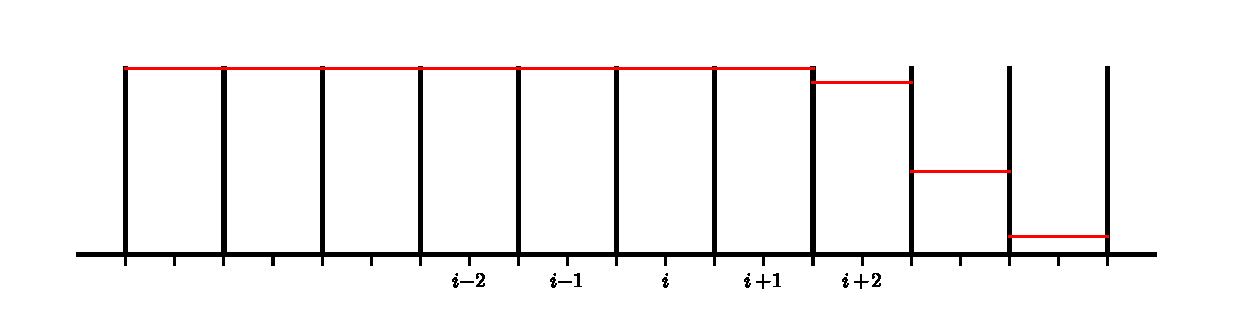
\includegraphics[width=0.55\linewidth]{rea-start_008} \\
\caption[The effect of limiters on initially discontinuous
  data]{\label{fig:limitingexb}Initially discontinuous data evolved
  for several steps with limiting.  Note that unlike the sequence
  without limiting (Figure~\ref{fig:limitingex}), the
  discontinuity remains sharper with limiting and there are no over-
  or undershoots.}
\end{figure}

A slightly more complex limiter is the MC limiter (monotonized central
difference).  First we define an extrema test,
\begin{equation}
\xi = (a_{i+1} - a_i) \cdot (a_i - a_{i-1})
\end{equation}
Then the limited difference is
\begin{equation}
\left . \frac{\partial a}{\partial x} \right |_i = 
 \left \{
\begin{array}{ll}
\min \left [ \frac{| a_{i+1} - a_{i-1} |}{2 \Delta x},
              2 \frac{| a_{i+1} - a_i |}{\Delta x},
              2 \frac{| a_{i} - a_{i-1} |}{\Delta x}
      \right ]  \mathrm{sign}(a_{i+1} - a_{i-1}) &  \xi > 0 \\
0 & \mathit{otherwise}
\end{array}
\right .
\end{equation}
%
Note that a slightly different form of this limiter is presented in
\cite{leveque:2002}, where all quantities are in a {\tt minmod}, which appears to limit a bit less.
This is second-order accurate for smooth flows.  

The main goal of a limiter is to reduce the slope near extrema.
Figure~\ref{fig:limit} shows a finite-volume grid with the original
data, cell-centered slopes, and MC limited slopes.  Note that near the
strong gradients is where the limiting kicks in.  The different limiters
are all constructed by enforcing a condition requiring the method to be
{\em total variation diminishing}, or TVD.  More details on TVD limiters
can be found in \cite{toro:1997,leveque:2002}.

% this figure can be create with figures/advection/generalgrid.py
\begin{figure}
\centering
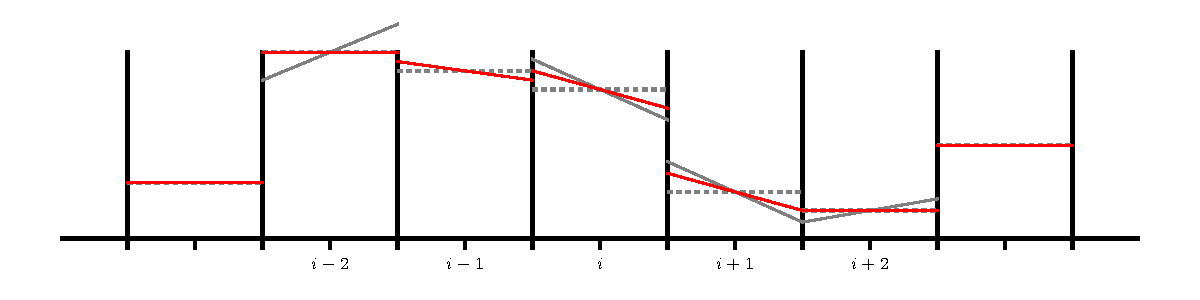
\includegraphics[width=\linewidth]{generalgrid}
\caption[Piecewise linear slopes with an without
  limiting]{\label{fig:limit} A finite-volume grid showing the cell
  averages (gray, dotted, horizontal lines), unlimited center-difference slopes
  (gray, solid) and MC limited slopes (red).  Note that in zones $i$ and
  $i+1$, the slopes are limited slightly, so as not to overshoot or
  undershoot the neighboring cell value.  Cell $i-1$ is not limited at
  all, whereas cells $i-2$, and $i+2$ are fully limited---the slope is
  set to 0---these are extrema.}
\end{figure}

A popular extension of the MC limiter is the $4^\mathrm{th}$-order MC
limiter, which is more accurate in smooth flows (this is shown in
\cite{colella:1985}, Eqs. 2.5 and 2.6; and \cite{colella:1990},
Eq. 191).

\begin{exercise}[Limiting and reduction in order-of-accuracy]
{Show analytically that if you fully limit the slopes
  (i.e.\ set $\partial a/\partial x |_i = 0$, that the second-order
  method reduces to precisely our first-order finite-difference discretization,
  Eq.~\ref{eq:fo}.  }
\end{exercise}

It is common to express the slope simply as the change in the state variable:
\begin{equation}
\Delta a_i = \left . \frac{\partial a}{\partial x} \right |_i \Delta x
\end{equation}
and to indicate the limited slope as $\overline{\Delta a}_i$.



%%%%%%%%%%%%%%%%%%%%%%%%%%%%%%%%%%%%%%%%%%%%%%%%%%%%%%%%%%%%%%%%%%%%%%%%%%%%%%
\subsection{Reconstruct-evolve-average}

Another way to think about these methods is as a reconstruction,
evolve, and average (R-E-A) process (see Figure~\ref{fig:rea}).  

We can write the conservative update as:
\begin{align}
a_i^{n+1} &= a_i^n + \frac{\Delta t}{\Delta x} 
    (u a^{n+\myhalf}_{i-\myhalf} - u a^{n+\myhalf}_{i+\myhalf} ) \\
          &= a_i^n + \cfl (a^{n+\myhalf}_{i-\myhalf} - a^{n+\myhalf}_{i+\myhalf} ) 
\end{align}
If we take $u > 0$, then the Riemann problem will always choose the
left state, so we can write this as:
\begin{equation}
a_i^{n+1} = a_i^n + 
     \cfl \biggl [\underbrace{\left (a_{i-1}^n + \frac{1}{2} (1-\cfl) \Delta a_{i-1} \right )}_{a_{i-\myhalf,L}} -
              \underbrace{\left (a_{i}^n + \frac{1}{2} (1-\cfl) \Delta a_{i} \right )}_{a_{i+\myhalf,L}}
       \biggr ] \label{eq:rea_orig}
\end{equation}

If we instead look at this via the R-E-A procedure, we write the reconstructed
$a$ in each zone in the form of a piecewise linear polynomial
\begin{equation}
a_i(x) = a_i + \frac{\Delta a_i}{\Delta x} (x - x_i)
\end{equation}
Consider zone $i$.  
If we are advecting with a CFL number $\cfl$, then that means that the fraction
$\cfl$ of the zone immediately to the left of the $i-\myhalf$ interface will advect
into zone $i$ over the timestep.  And only the fraction $1-\cfl$ in zone $i$
immediately to the right of the interface will stay in that zone.  This 
is indicated by the shaded regions in Figure~\ref{fig:rea}. 

The average of the quantity $a$ from zone $i-1$ that will advect into
zone $i$ is 
\begin{eqnarray}
\mathcal{I}_< &=& \frac{1}{\cfl \Delta x} 
   \int_{x_{i-\myhalf} - \cfl\Delta x}^{x_{i-\myhalf}} a_{i-1}(x) dx \\
%
 &=& \frac{1}{\cfl \Delta x} 
   \int_{x_{i-\myhalf} - \cfl\Delta x}^{x_{i-\myhalf}}
        \left [ a_{i-1} + \frac{\Delta a_{i-1}}{\Delta x} (x - x_{i-1} ) \right ] dx  \\
 &=& a_{i-1} + \frac{1}{2} \Delta a_{i-1} (1-\cfl)
\end{eqnarray}

And the average of the quantity $a$ in zone $i$ that will remain in zone $i$
is
\begin{eqnarray}
\mathcal{I}_> &=& \frac{1}{(1-\cfl) \Delta x} 
   \int_{x_{i-\myhalf}}^{x_{i-\myhalf} + (1-\cfl) \Delta x} a_{i}(x) dx \\
%
 &=& \frac{1}{(1-\cfl) \Delta x} 
   \int_{x_{i-\myhalf}}^{x_{i-\myhalf} + (1-\cfl)\Delta x} 
        \left [ a_{i} + \frac{\Delta a_{i}}{\Delta x} (x - x_{i} ) \right ] dx  \\
 &=& a_{i} - \frac{1}{2} \Delta a_{i} \cfl
\end{eqnarray}

The final part of the R-E-A procedure is to average the over the 
advected profiles in the new cell.  The weighted average of the
amount brought in from the left of the interface and that that remains
in the cell is
\begin{align}
a_i^{n+1} &= \cfl \mathcal{I}_< + (1 - \cfl) \mathcal{I}_>  \\
          &= \cfl \left [ a^n_{i-1} + \frac{1}{2} \Delta a_{i-1} (1 - \cfl) \right ]
   + (1-\cfl) \left [ a^n_i - \frac{1}{2} \Delta a_i \cfl \right ] \\
          &= a^n_i + \cfl \left [a^n_{i-1} + \frac{1}{2}(1 - \cfl) \Delta a_{i-1} \right ]
           - \cfl \left [ a^n_i + \frac{1}{2} (1-\cfl) \Delta a_i \right ]
\end{align}          
This is identical to Eq.~\ref{eq:rea_orig}.  This demonstrates that the
R-E-A procedure is equivalent to our reconstruction, prediction of the
interface states, solving the Riemann problem, and doing the 
conservative flux update.

% this figure sequence is created by figures/advection/rea.py
\begin{figure}
\centering
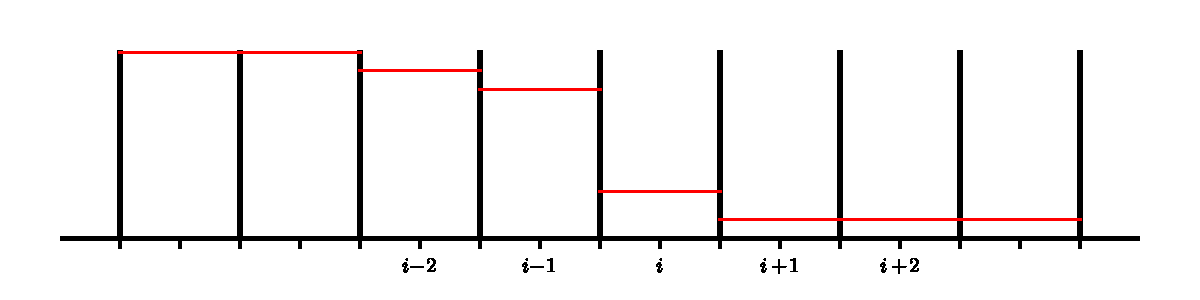
\includegraphics[width=\linewidth]{rea-start} \\
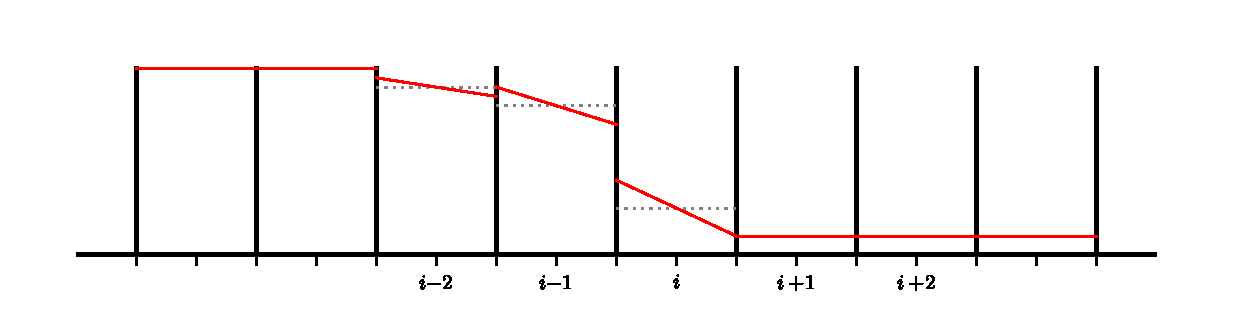
\includegraphics[width=\linewidth]{rea-reconstruction} \\
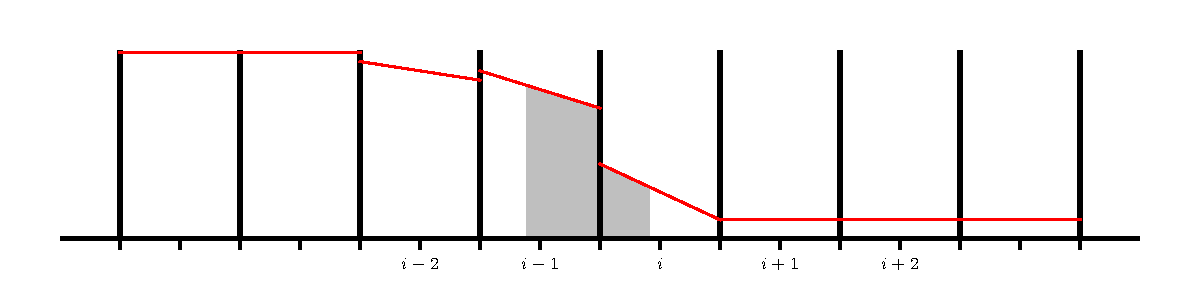
\includegraphics[width=\linewidth]{rea-trace} \\
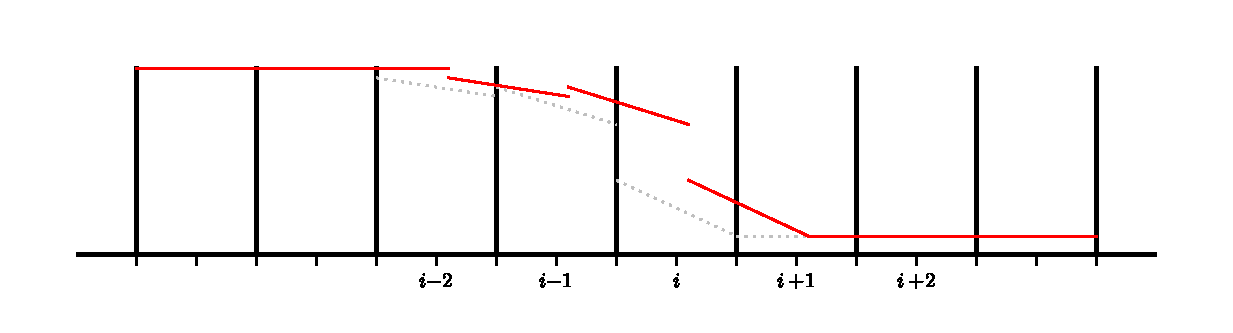
\includegraphics[width=\linewidth]{rea-evolve} \\
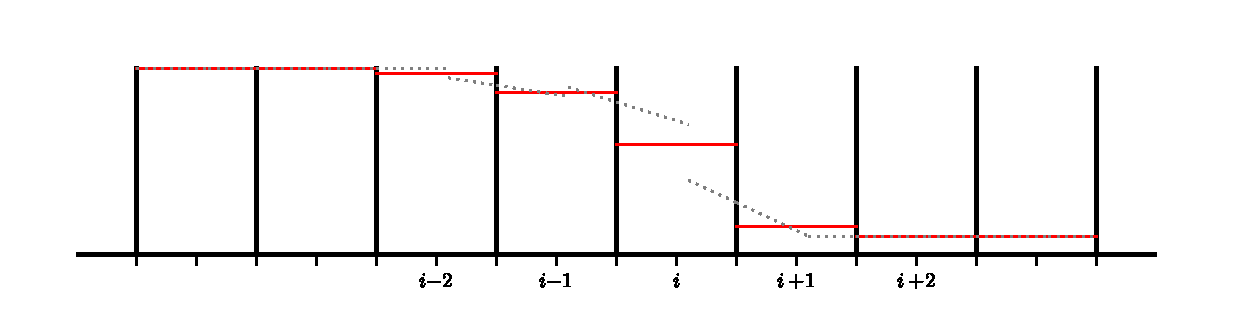
\includegraphics[width=\linewidth]{rea-final}
\caption[The Reconstruct-Evolve-Average procedure]{\label{fig:rea}
  Reconstruct-Evolve-Average.  The top panel shows the original
  cell-average data.  The second panel shows the (limited) piecewise
  linear reconstruction of the data.  Assuming a CFL number of 0.6 and
  advection to the right, the shaded regions in the third panel show
  the data that will wind up in cell $i$ after advecting for a single
  step.  The fourth panel shows the piecewise-linear data advected to
  the right by 0.6 of a cell-width (corresponding to a CFL of 0.6).
  The final panel shows the new averages of the data, constructed by
  averaging the advected piecewise linear data in each cell.}
\end{figure}




%%%%%%%%%%%%%%%%%%%%%%%%%%%%%%%%%%%%%%%%%%%%%%%%%%%%%%%%%%%%%%%%%%%%%%%%%%%%%%
\section{Errors and convergence rate}

For the advection problem (with $u>0$), the analytic solution is to
simply propagate the initial profile to the right.  This means that
with periodic boundary conditions, after advecting for one period, our
numerical solution should be identical to the initial conditions.  Any
differences are our numerical error.  We can quantify the error by
taking the norm of error\footnote{see \S~\ref{intro:sec:norm} for the
  definition of the norms} as:
\begin{equation}
\epsilon^\mathrm{abs} = \| a^\mathrm{final} - a^\mathrm{init} \|_2 \equiv
   \left [ \frac{1}{N} \sum_{i=1}^N 
   ( a_i^\mathrm{final} - a_i^\mathrm{init} )^2
  \right ]^{\myhalf}
\end{equation}
It is sometimes useful to compare to the norm of the original solution
to get a measure of the relative error:
\begin{equation}
\epsilon^\mathrm{rel} \equiv \frac{\| a^\mathrm{final} - a^\mathrm{init} \|_2}
   {\| a^\mathrm{init} \|_2}
\end{equation}
Note that for the absolute norm, it is important in these definitions
to normalize by the number of zones, $N$, otherwise our error will be
resolution-dependent.  For the relative norm, since we scale by a norm
on the same grid, this normalization will cancel.
%
\begin{exercise}[Convergence testing]
{ Run the first-order solver for several different values of $\Delta x$,
each a factor of 2 smaller than the previous.  Compute $\epsilon$ for
each resolution and observe that it converges in a first-order fashion
(i.e.\ $\epsilon$ decreases by 2 when we decrease $\Delta x$ by a factor of 2).

\noindent Do the same with the second-order solver and observe that it
converges as second-order. However: you may find less than
second-order if your initial conditions have discontinuities and you
are limiting.  Figure~\ref{fig:advnorm} shows the convergence of the
method with no limiting, MC, and minmod limiting, $\cfl = 0.8$, and a
Gaussian initial condition for 5 periods.}
\end{exercise}

% figure from hydro_examples: advection/advection.py
\begin{figure}[t]
\centering
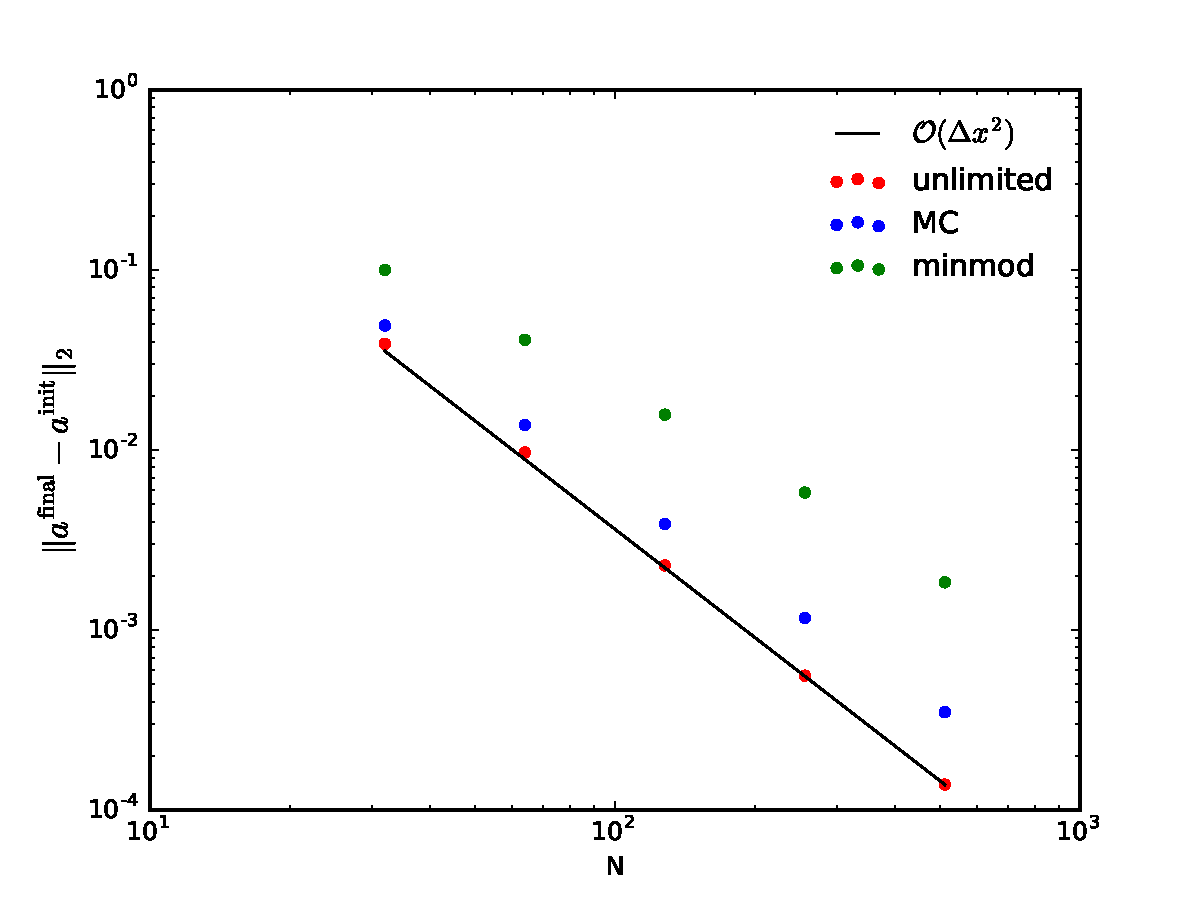
\includegraphics[width=0.8\linewidth]{plm-converge}
\caption[Convergence of second-order finite-volume advection]
        {\label{fig:advnorm} Convergence for the second-order
          finite-volume method with no limiting, MC, and minmod limiting advecting a
          Gaussian initial profile with $\cfl = 0.8$ for 5 periods. \\
        \hydroexdoit{\href{https://github.com/zingale/hydro_examples/blob/master/advection/advection.py}{advection.py}}}
\end{figure}

\begin{figure}[ht]
\centering
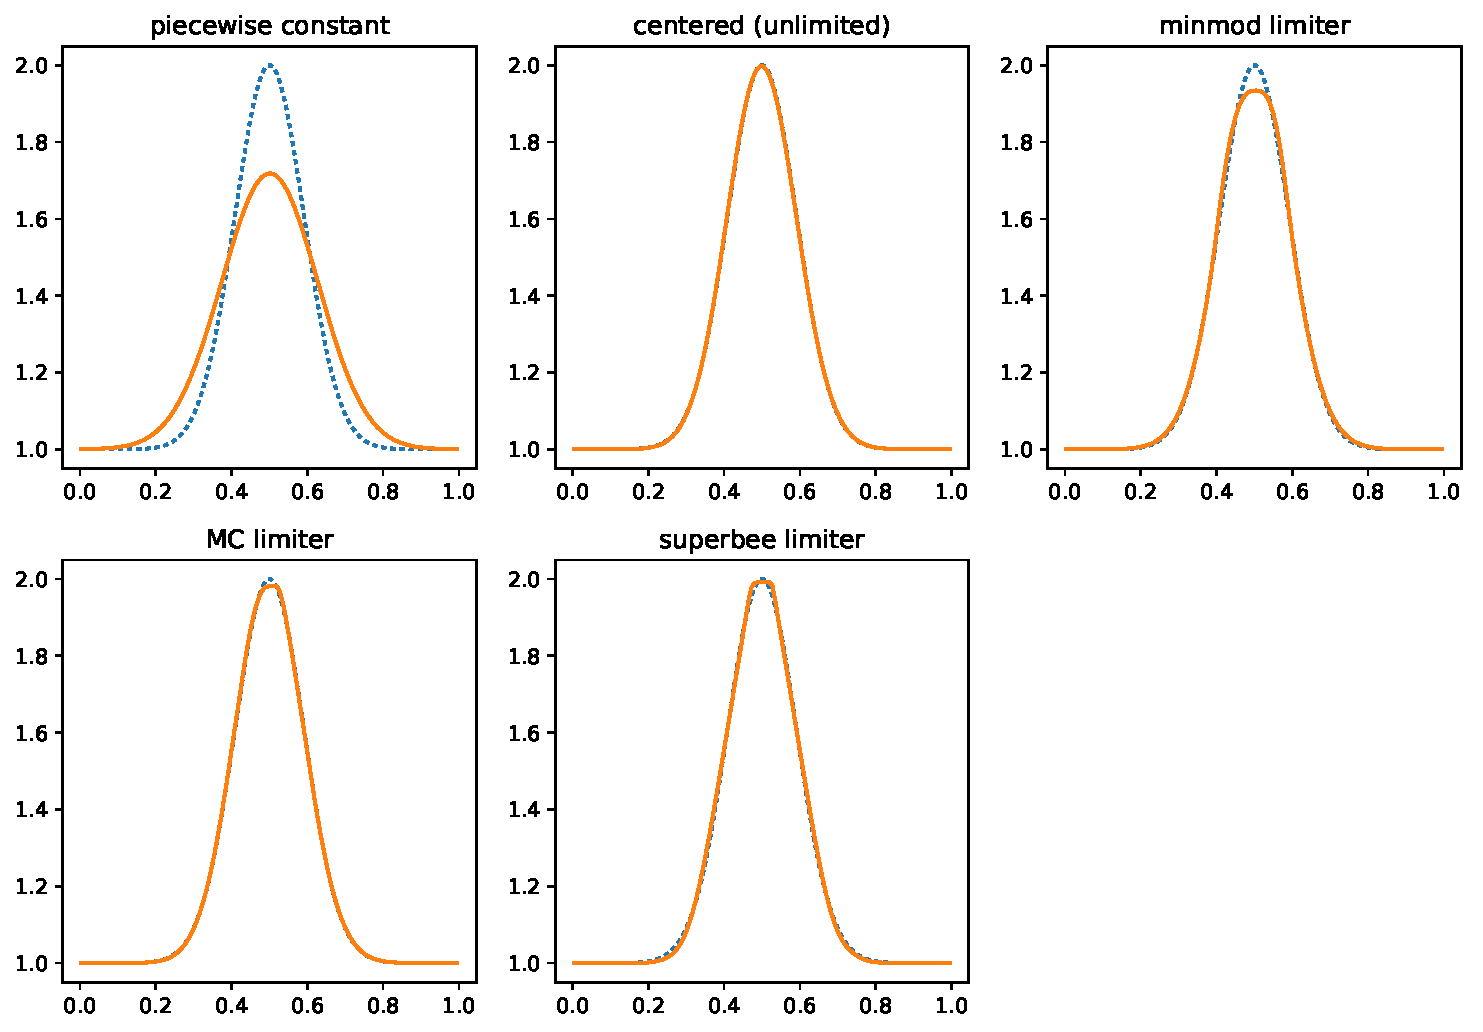
\includegraphics[width=0.8\linewidth]{fv-gaussian-limiters} \\[1em]
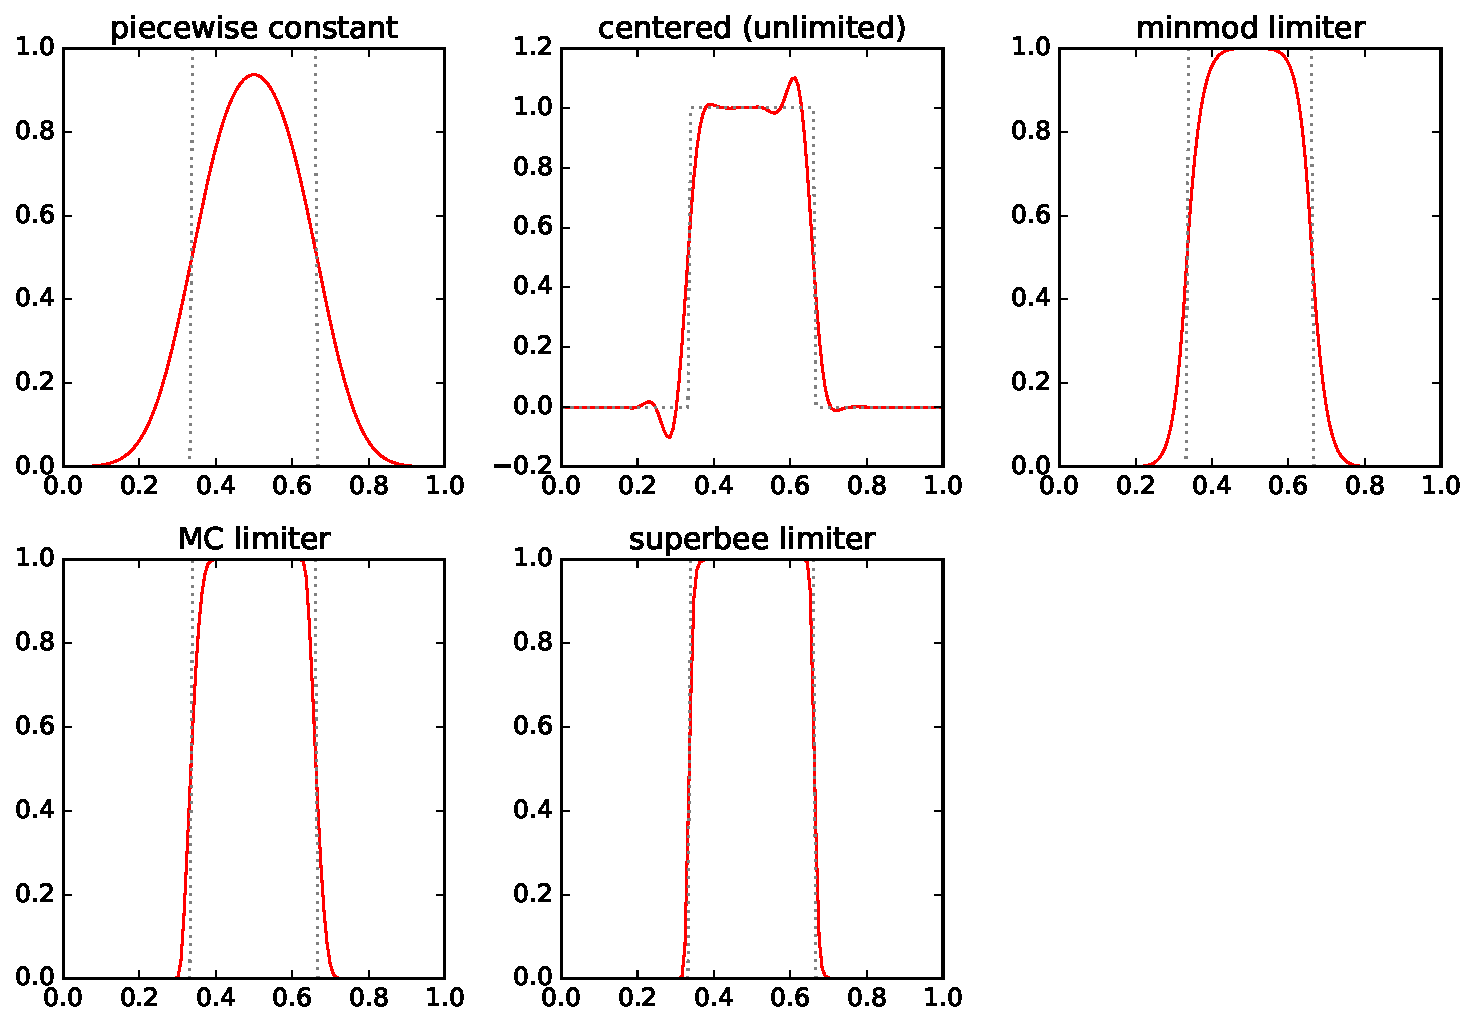
\includegraphics[width=0.8\linewidth]{fv-tophat-limiters} 
\caption[Effect of different limiters on evolution]
        {\label{fig:limiter_panel} The effect of different limiters on the
          evolution of a Gaussian initial profile (top) and a tophat initial
          profile (bottom), using $\cfl = 0.8$ and 5 periods. \\
        \hydroexdoit{\href{https://github.com/zingale/hydro_examples/blob/master/advection/advection.py}{advection.py}}}
\end{figure}

As seen in figure~\ref{fig:advnorm}, the choice of limiters can have a great
effect on the accuracy.  Figure~\ref{fig:limiter_panel} shows the Gaussian and
tophat profiles with several different limiters.

\section{Multi-dimensional advection}

The two-dimensional linear advection equation is:
\begin{equation}
a_t + u a_x + v a_y = 0
\label{eq:advect2d}
\end{equation}
where $u$ is the velocity in the $x$-direction and $v$ is the velocity in
the $y$-direction.  We denote the average of $a(x,y,t)$ in a zone $i,j$ as
$a_{i,j}$.  Here, $i$ is the index in the $x$-direction and $j$ is the
index in the $y$-direction.  A 2-d grid is shown in Figure~\ref{fig:2dgrid}.
Just as in the one-dimensional case, we will extend the domain with a
perimeter of ghost cells to set the boundary conditions.

% this is create by figures/advection/2dgrid.py
\begin{figure}[h]
\centering
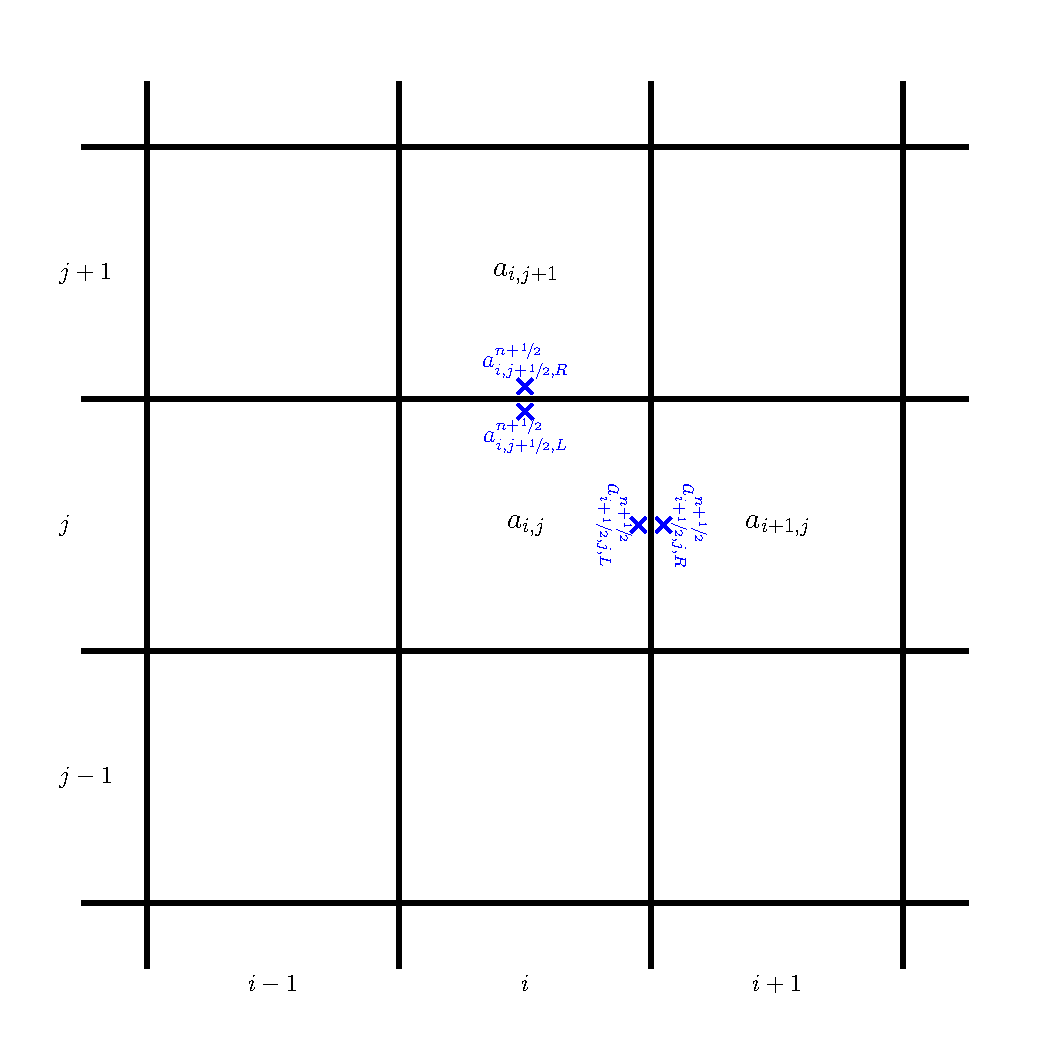
\includegraphics[width=4.0in]{2dgrid}
\caption[A 2-d grid with zone-centered indexes]{\label{fig:2dgrid} A
  simple 2-d grid with the zone-centered indexes.  The $\times$s mark
  the left and right interface states at the upper edge of the $i,j$ zone in each
  coordinate direction.  For a finite-volume discretization, $a_{i,j}$ 
  represents the average of $a(x,y)$ over the zone.}
\end{figure}

To derive the finite-volume form of the update, we start by writing
this in conservative form.  Since $u$ and $v$ are constant, we can
move them inside the divergences:
\begin{equation}
a_t + (u a)_x + (v a)_y = 0
\label{eq:advect2d-cons}
\end{equation}
This is the form we will integrate over zones.  As before, we will
define the average of $a$ in a zone by integrating it over the
volume:
\begin{equation}
a_{i,j} = \frac{1}{\Delta x \Delta y} 
   \int_{x_{i-\myhalf}}^{x_{i+\myhalf}} \int_{y_{j-\myhalf}}^{y_{j+\myhalf}} 
   a(x,y,t) \, dx \, dy
\end{equation}
Integrating Eq.~\ref{eq:advect2d-cons} over $x$ and $y$, we have:
\begin{align}
\frac{1}{\Delta x \Delta y} 
  \int_{x_{i-\myhalf}}^{x_{i+\myhalf}} 
  \int_{y_{j-\myhalf}}^{y_{j+\myhalf}} a_t \, dx \, dy =  
  &- \frac{1}{\Delta x \Delta y}
       \int_{x_{i-\myhalf}}^{x_{i+\myhalf}} \int_{y_{j-\myhalf}}^{y_{j+\myhalf}}
      (u a)_x \, dx \, dy \nonumber \\
  &- \frac{1}{\Delta x \Delta y}
       \int_{x_{i-\myhalf}}^{x_{i+\myhalf}} \int_{y_{j-\myhalf}}^{y_{j+\myhalf}}
      (v a)_y \, dx \, dy 
\end{align}
or using the divergence theorem,
\begin{align}
\label{eq:adv:multiddivergence}
 \frac{\partial a_{i,j}}{\partial t} =
  &- \frac{1}{\Delta x\Delta y} \int_{y_{j-\myhalf}}^{y_{j+\myhalf}}
     \left \{ (u a)_{i+\myhalf,j} - (u a)_{i-\myhalf,j} \right \} dy \nonumber \\
  &- \frac{1}{\Delta x\Delta y} \int_{x_{i-\myhalf}}^{x_{i+\myhalf}}
     \left \{ (v a)_{i,j+\myhalf} - (v a)_{i,j-\myhalf} \right \} dx
\end{align}

Now we integrate over time---the left side of our expression becomes
just the difference between the new and old state.
\begin{align}
 a_{i,j}^{n+1} - a_{i,j}^n = 
  &- \frac{1}{\Delta x\Delta y} \int_{t^n}^{t^{n+1}} \int_{y_{j-\myhalf}}^{y_{j+\myhalf}}
     \left \{ (u a)_{i+\myhalf,j} - (u a)_{i-\myhalf,j} \right \} dy dt \nonumber \\
  &- \frac{1}{\Delta x\Delta y} \int_{t^n}^{t^{n+1}} \int_{x_{i-\myhalf}}^{x_{i+\myhalf}}
     \left \{ (v a)_{i,j+\myhalf} - (v a)_{i,j-\myhalf} \right \} dx dt
\label{eq:update2du}
\end{align}
We define the flux through the interface as the average over the face
of that interface and time: \MarginPar{is there a way to illustrate this, as some space-time diagram?}
\begin{itemize}
\item x-face:
\begin{equation}
\langle (ua)_{i+\myhalf,j}\rangle_{(t)} = \frac{1}{\Delta y \Delta t}
    \int_{t^n}^{t^{n+1}} \int_{y_{j-\myhalf}}^{y_{j+\myhalf}} (ua)_{i+\myhalf,j}\, dy dt
\end{equation}
\item y-face
\begin{equation}
\langle (va)_{i,j+\myhalf}\rangle_{(t)} = \frac{1}{\Delta x \Delta t}
    \int_{t^n}^{t^{n+1}} \int_{x_{i-\myhalf}}^{x_{i+\myhalf}} (va)_{i,j+\myhalf}\, dx dt 
\end{equation}
\end{itemize}
where $\langle . \rangle_{(t)}$ denotes the time-average over the face.
For a second-order accurate method in time, we replace the average in
time with the flux at the midpoint in time and the average over the face
with the flux at the center of the face: 
\begin{equation}
\langle (ua)_{i+\myhalf,j} \rangle_{(t)} \approx (ua)_{i+\myhalf,j}^{n+\myhalf}
\end{equation}
Then we have:
\begin{equation}
a_{i,j}^{n+1} = a_{i,j}^n - \Delta t \left [
   \frac{(ua)_{i+\myhalf,j}^{n+\myhalf} - (ua)_{i-\myhalf,j}^{n+\myhalf}}{\Delta x} +
   \frac{(va)_{i,j+\myhalf}^{n+\myhalf} - (va)_{i,j-\myhalf}^{n+\myhalf}}{\Delta y} \right ]
\end{equation}

For the advection problem, since $u$ and $v$ are constant, we need
to find the interface states of $a$ alone.
There are two methods for computing these interface states, 
$a_{i\pm\myhalf,j}^{n+\myhalf}$ on $x$-interfaces and  $a_{i,j\pm\myhalf}^{n+\myhalf}$ on $y$-interfaces:
dimensionally split and unsplit.  Dimensionally split methods are
easier to code, since each dimension is operated on independent of the
others, so you can simply call a one-dimensional method for each
direction.  Unsplit methods, however, are more accurate and less
susceptible to grid effects.  \MarginPar{show an example + refs? Zalesak test?}

\subsection{Dimensionally split}

In a split method, we update the state in each coordinate direction
independently.  This is simple and a straightforward way to use
one-dimensional methods in multi-d.  To be second-order accurate in
time, we do {\em Strang splitting}~\cite{strang}, where we alternate
the order of the dimensional updates each timestep.  An update through
$\Delta t$ consists of $x$ and $y$ sweeps and appears as:
\begin{eqnarray}
 \frac{a_{i,j}^\star - a_{i,j}^n}{\Delta t} &=&
  - \frac{ u a_{i+\myhalf,j}^{n+\myhalf} - u a_{i-\myhalf,j}^{n+\myhalf} }{\Delta x} \label{eq:splitx}\\
 \frac{a_{i,j}^{n+1} - a_{i,j}^\star}{\Delta t} &=&
  - \frac{ v a_{i,j+\myhalf}^{\star,n+\myhalf} - v a_{i,j-\myhalf}^{\star,n+\myhalf} }{\Delta y} \label{eq:splity}
\end{eqnarray}
Here, Eq.~\ref{eq:splitx} is the update in the $x$-direction.  In
constructing the interface states, $a_{i+\myhalf,j}^{n+\myhalf}$ and
$a_{i-\myhalf,j}^{n+\myhalf}$, we do the exact same procedure as the
one-dimensional case, constructing the left and right states at each
interface and then solving the same Riemann problem to find the unique
state on the interface.  Each dimensional sweep is done without
knowledge of the other dimensions.  For example, in the $x$-update, we
are solving:
\begin{equation}
a_t + u a_x = 0
\label{eq:advect1dx}
\end{equation}
and in the $y$-update, we are solving:
\begin{equation}
a_t + v a_y = 0
\end{equation}

The construction of the interface states largely mimics the one-dimensional
case (Eq.~\ref{eq:statel} and \ref{eq:stater}).  For example, the
$a_{i+\myhalf,j,L}^{n+\myhalf}$ state is:
\begin{eqnarray}
a_{i+\myhalf,j,L}^{n+\myhalf} &=& a_{i,j}^n + 
  \frac{\Delta x}{2} \left .\frac{\partial a}{\partial x} \right |_{i,j} + 
  \frac{\Delta t}{2} \left .\frac{\partial a}{\partial t} \right |_{i,j} + 
  \mathcal{O}(\Delta x^2) + \mathcal{O}(\Delta t^2) \nonumber \\
 &=& a_{i,j}^n + 
   \frac{\Delta x}{2} \left .\frac{\partial a}{\partial x} \right |_{i,j} + 
   \frac{\Delta t}{2} \left ( 
   - u \left .\frac{\partial a}{\partial x} \right |_{i,j} \right
   ) + \ldots \nonumber \\
    &=& a_{i,j}^n + 
   \frac{\Delta x}{2} \left ( 1 - \frac{\Delta t}{\Delta x} u \right ) 
   \left .\frac{\partial a}{\partial x} \right |_{i,j} +
   \ldots \label{eq:statels}
\end{eqnarray}
Notice that when substituting for $\partial a / \partial t$, we use
the one-dimensional split version of the advection equation
(Eq.~\ref{eq:advect1dx}) instead of the full multi-dimensional
equation.  There are no $y$-direction terms that come into play in the
split method when considering the $x$-direction.

The $x$-update
(Eq.~\ref{eq:splitx}) updates the state only accounting for the
$x$-fluxes---we denote this intermediate state with the `$\star$'
superscript.  For the $y$-update, we construct our interface states in
the analogous way as in the $x$-direction, but begin with the `$\star$'
state instead of the old-time state.  In this fashion, the $y$-update
`sees' the result of the $x$-update and couples things together.

To achieve second-order accuracy in time, it is necessary to alternate
the directions of the sweeps each timestep, i.e., $x$-$y$ then $y$-$x$.
Furthermore, this pair of sweeps should use the same timestep, $\Delta t$.


\subsection{Unsplit multi-dimensional advection}
\label{adv:sec:unsplit_2d}

The unsplit case differs from the dimensionally split case in two
ways: (1) in predicting the interface states, we use knowledge of the
flow in the transverse direction, and (2), only a single conservative
update is done per timestep, with all directions updating
simultaneously.  See \cite{colella:1990} for more details.  This idea
is sometimes called the ``corner transport upwind'' or CTU method.

The construction of the $a_{i+\myhalf,j,L}^{n+\myhalf}$ interface state appears as
\begin{eqnarray}
a_{i+\myhalf,j,L}^{n+\myhalf} &=& a_{i,j}^n + 
  \frac{\Delta x}{2} \left .\frac{\partial a}{\partial x} \right |_{i,j} + 
  \frac{\Delta t}{2} \left .\frac{\partial a}{\partial t} \right |_{i,j} + 
  \mathcal{O}(\Delta x^2) + \mathcal{O}(\Delta t^2) \nonumber \\
 &=& a_{i,j}^n + 
   \frac{\Delta x}{2} \left .\frac{\partial a}{\partial x} \right |_{i,j} + 
   \frac{\Delta t}{2} \left ( 
   - u \left .\frac{\partial a}{\partial x} \right |_{i,j} 
   - v \left .\frac{\partial a}{\partial y} \right |_{i,j} \right
   ) + \ldots \nonumber \\
    &=& \underbrace{a_{i,j}^n + 
   \frac{\Delta x}{2} \left ( 1 - \frac{\Delta t}{\Delta x} u \right ) 
   \left .\frac{\partial a}{\partial x} \right |_{i,j}}_{\hat{a}_{i+\myhalf,j,L}^{n+\myhalf}} \underbrace{-
   \frac{\Delta t}{2} v \left .\frac{\partial a}{\partial y} \right |_{i,j}}_{\mathrm{``transverse~flux~difference''}} +
   \ldots \label{eq:statelu}
\end{eqnarray}
The main difference between the split and unsplit interface states is the
explicitly appearance of the ``transverse flux difference'' in the unsplit
interface state.  We rewrite this as:
\begin{equation}
a_{i+\myhalf,j,L}^{n+\myhalf} = \hat{a}_{i+\myhalf,j,L}^{n+\myhalf} 
   - \frac{\Delta t}{2} v \left .\frac{\partial a}{\partial y} \right |_{i,j}
\end{equation}
Here, the $\hat{a}_{i+\myhalf,j,L}^{n+\myhalf}$ term is just the normal
prediction without considering the transverse direction (e.g., Eq.~\ref{eq:statels}).  The basic
update procedure is:
\begin{itemize}
\item Construct the normal predictor term, $\hat{a}_{i+\myhalf,j,L}^{n+\myhalf}$,
in a fashion identical to the one-dimensional and split methods.  We
compute these one-dimensional $\hat{a}$'s at the left and right every
interface in both coordinate directions.  Note that these states are
still one-dimensional, since we have not used any information from the
transverse direction in their computation.  

\item Solve a Riemann problem at each of these interfaces:
\begin{eqnarray}
a^T_{i+\myhalf,j} &=& \mathcal{R}(\hat{a}_{i+\myhalf,j,L}^{n+\myhalf},
                              \hat{a}_{i+\myhalf,j,R}^{n+\myhalf}) \\
a^T_{i,j+\myhalf} &=& \mathcal{R}(\hat{a}_{i,j+\myhalf,L}^{n+\myhalf},
                              \hat{a}_{i,j+\myhalf,R}^{n+\myhalf}) \\
\end{eqnarray}
These states are given the `$^T$' superscript since they are the states
that are used in computing the transverse flux difference.  

\item Correct the 
previously computed normal interface states (the $\hat{a}$'s) with
the transverse flux difference:
\begin{equation}
a_{i+\myhalf,j,L}^{n+\myhalf} = \hat{a}_{i+\myhalf,j,L}^{n+\myhalf} 
   - \frac{\Delta t}{2} v \frac{a^T_{i,j+\myhalf} - a^T_{i,j-\myhalf}}{\Delta y}
\end{equation}
Notice that the
fluxes that are differenced for the left state are those that are
transverse, but to the left of the interface.  Similarly, for the
right state, it would be those that are transverse, but to the right
of the interface:
\begin{equation}
a_{i+\myhalf,j,R}^{n+\myhalf} = \hat{a}_{i+\myhalf,j,R}^{n+\myhalf} 
   - \frac{\Delta t}{2} v \frac{a^T_{i+1,j+\myhalf} - a^T_{i+1,j-\myhalf}}{\Delta y}
\end{equation}
\end{itemize}
A similar procedure happens at the $y$-interfaces.  

Figure~\ref{fig:unsplitstates} illustrates the steps involved in
the construction of the $a_{i+\myhalf,j,L}^{n+\myhalf}$ state.  \MarginPar{more panels illustrating the sequence?}
%
% this is created by figures/advection/2dgrid-hat.py
% and                                  2dgrid-transverse.py
\begin{figure}
\centering
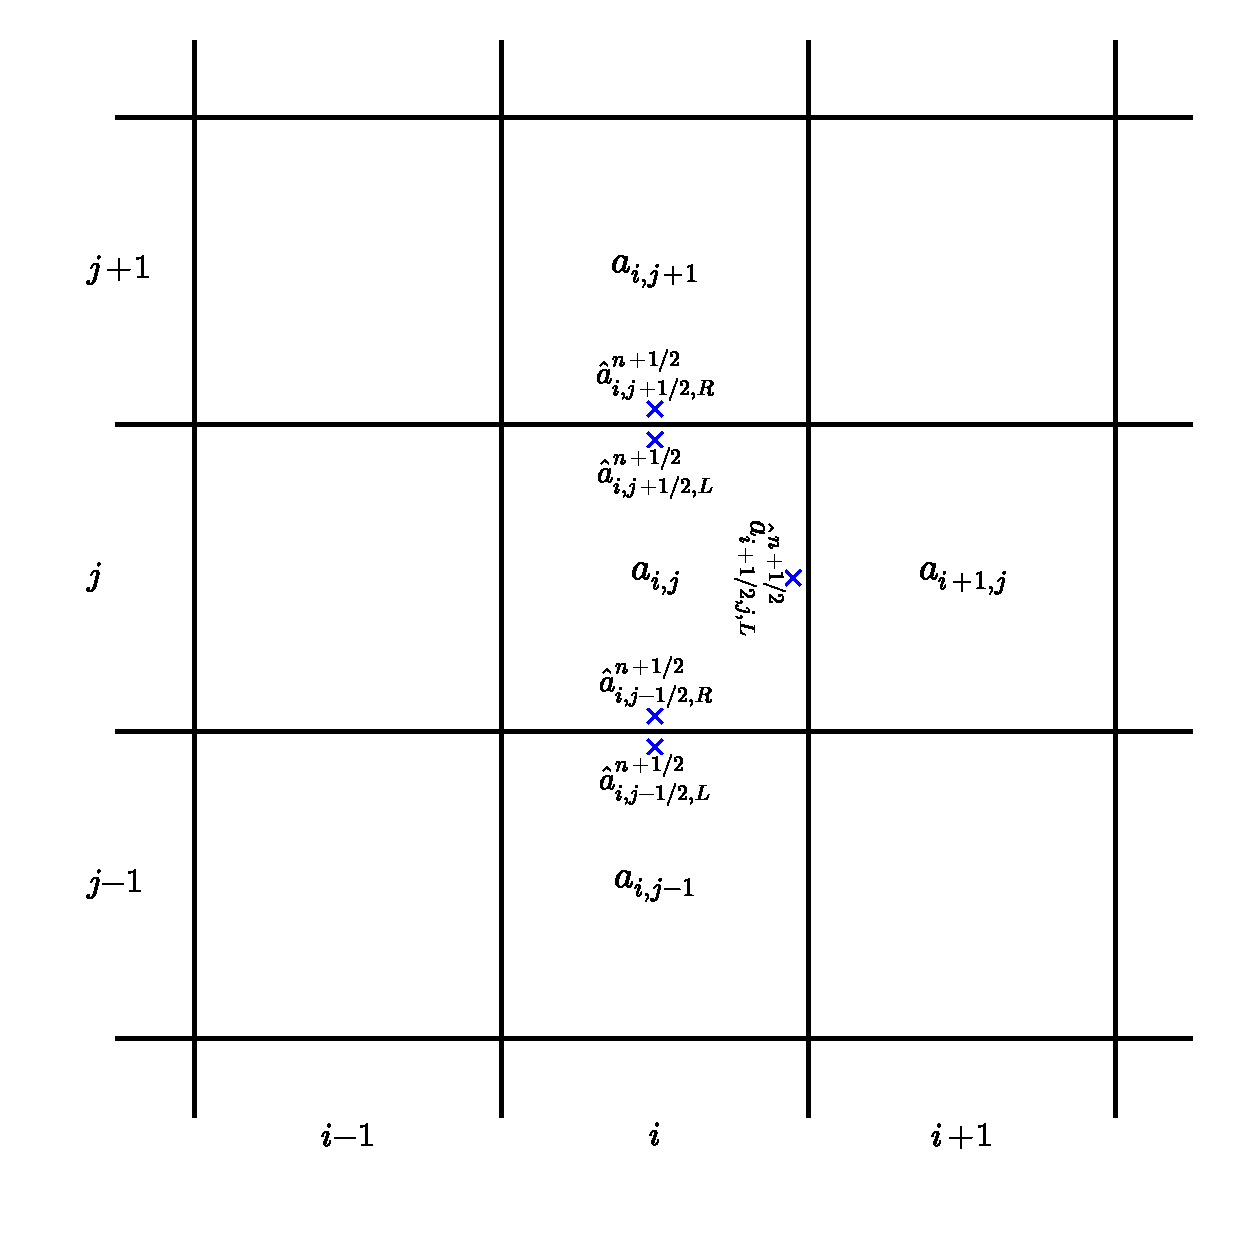
\includegraphics[width=0.7\linewidth]{2dgrid-hat} \\
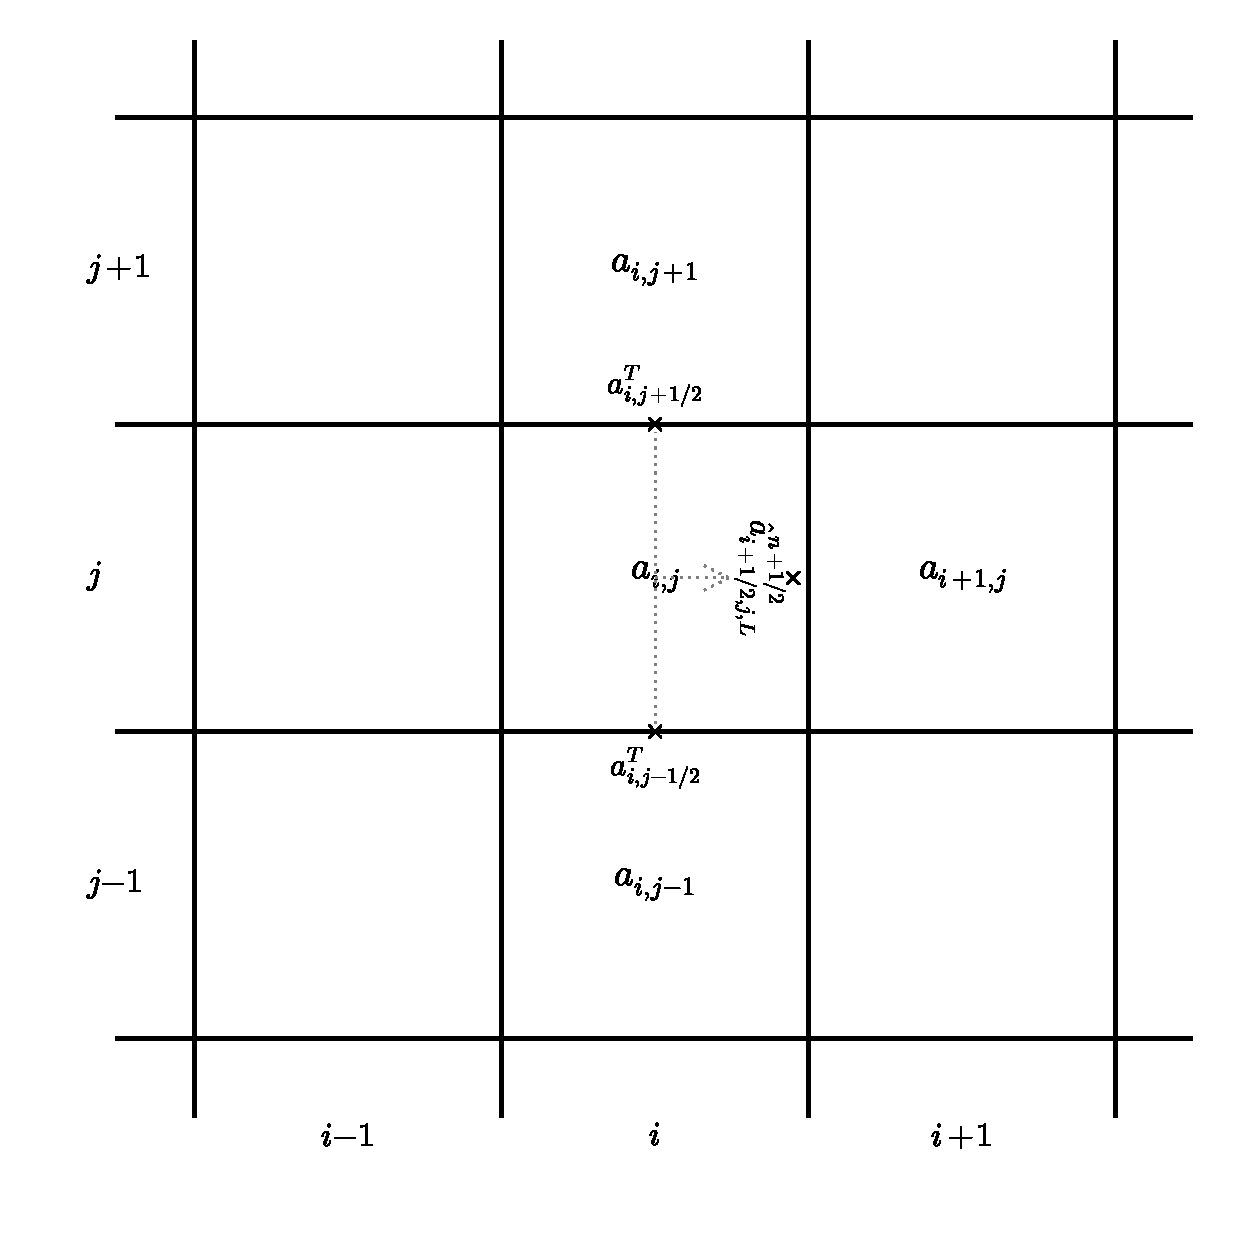
\includegraphics[width=0.7\linewidth]{2dgrid-transverse}
\caption[The construction of an interface state with the transverse
  component]{\label{fig:unsplitstates} The construction of the
  $a_{i+\myhalf,j,L}^{n+\myhalf}$ state.  Top: first we compute the
  $\hat{a}$'s---here we show all of the $\hat{a}$'s that will be used
  in computing the full left interface state at $(i+\myhalf,j)$.  Bottom:
  after the transverse Riemann solves, we have the two transverse
  states ($a^T_{i,j+\myhalf}$ and $a^T_{i,j-\myhalf}$) that will be
  differenced and used to correct $\hat{a}_{i+\myhalf,j,L}^{n+\myhalf}$
  (illustrated by the dotted lines) to make $a_{i+\myhalf,j,L}^{n+\myhalf}$.}
\end{figure}

Once all of the full states (normal prediction $+$ transverse flux
difference) are computed to the left and right of all the interfaces
($x$ and $y$), we solve another Riemann problem to find the final 
state on each interface.
\begin{equation}
a_{i+\myhalf,j}^{n+\myhalf} = \mathcal{R}(a_{i+\myhalf,j,L}^{n+\myhalf},
                                  a_{i+\myhalf,j,R}^{n+\myhalf}) \\
\end{equation}
The final conservative update is then done via Eq.~\ref{eq:update2du}.

See \cite{colella:1990} for more details on this unsplit method, 
and \cite{saltzman:1994} for details of the extension to 3-d.

Figures~\ref{fig:adv:gaussian-2d} and \ref{fig:adv:tophat-2d} show the
advection of a smooth Gaussian and a discontinuous tophat diagonally on
a coarse $32\times 32$ zone domain.  Each show a diffusion of the
initial function, similar to what we saw in 1-d.  In the tophat, we
also see a slight undershoot on the trailing side of the tophat after
one period.




% run as: ./pyro.py advection smooth inputs.smooth
% visualized as: ./plot.py -W 7.7 -H 6 -o smooth_init.pdf advection smooth_0000
\begin{figure}
\centering
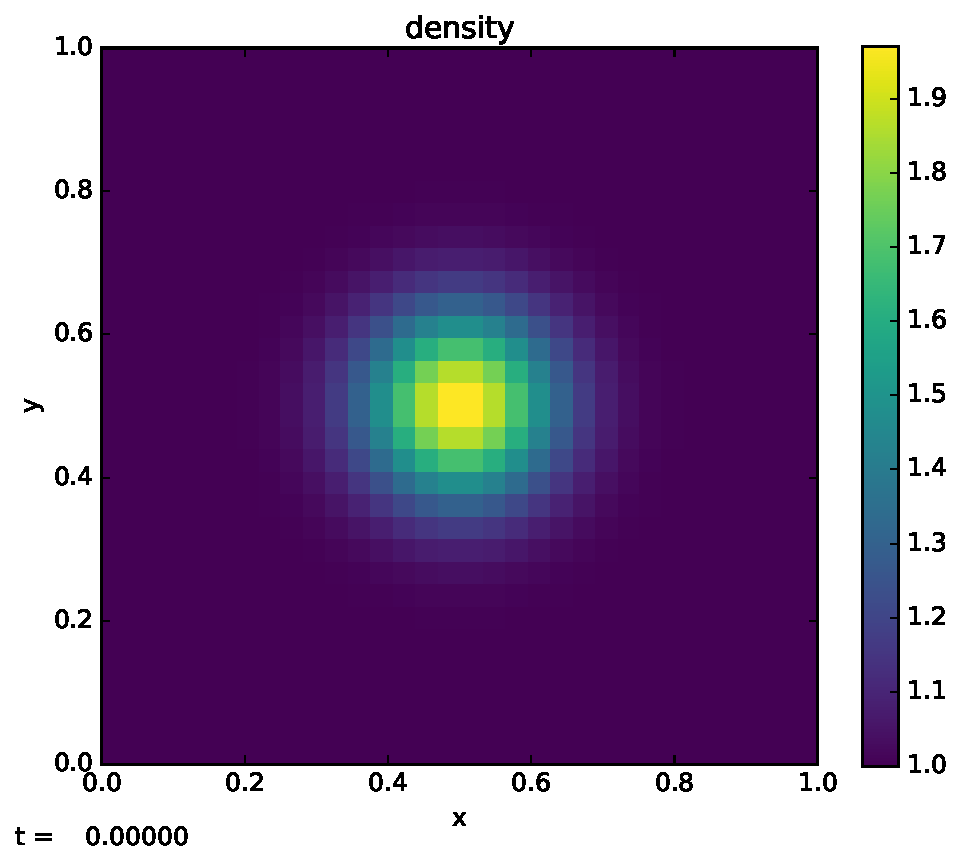
\includegraphics[width=0.48\linewidth]{smooth_init}\hspace{1em}
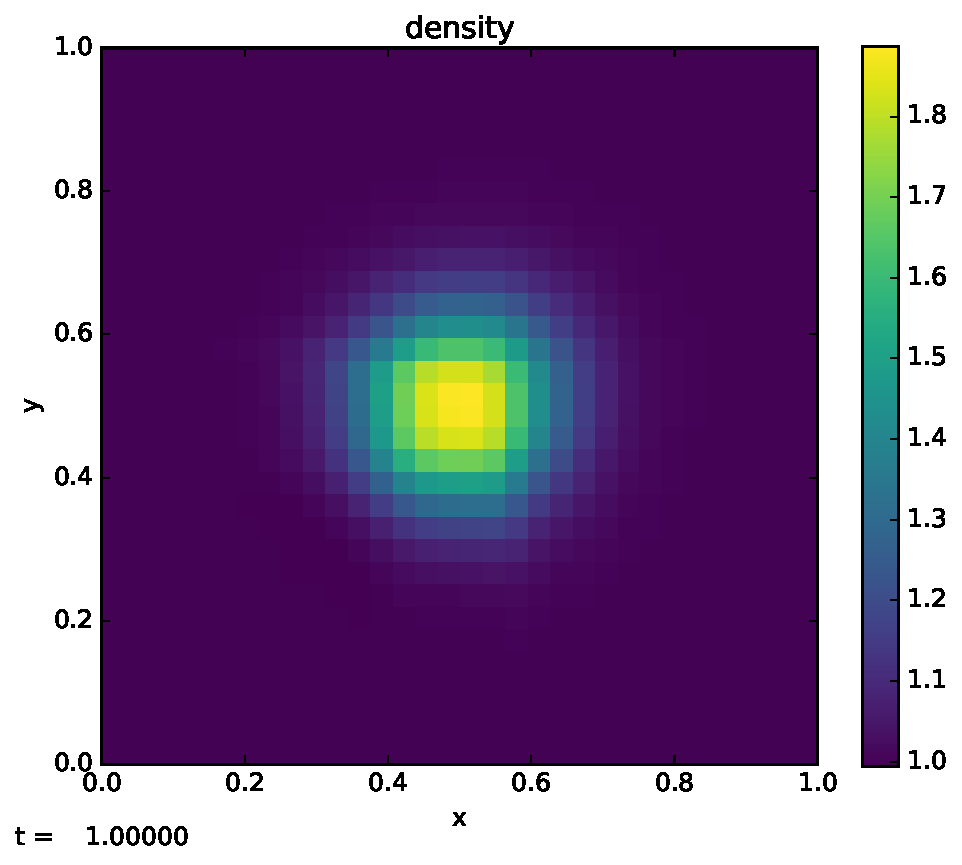
\includegraphics[width=0.48\linewidth]{smooth_final}
\caption[Advection of Gaussian profile in 2-d]
  {\label{fig:adv:gaussian-2d} Advection of a Gaussian profile
  with $u = v = 1$ for one period on a $32\times 32$ grid, with $\cfl =
  0.8$.  This was run with \pyro\ as {\tt ./pyro.py advection smooth
    inputs.smooth}}
\end{figure}

\begin{figure}
\centering
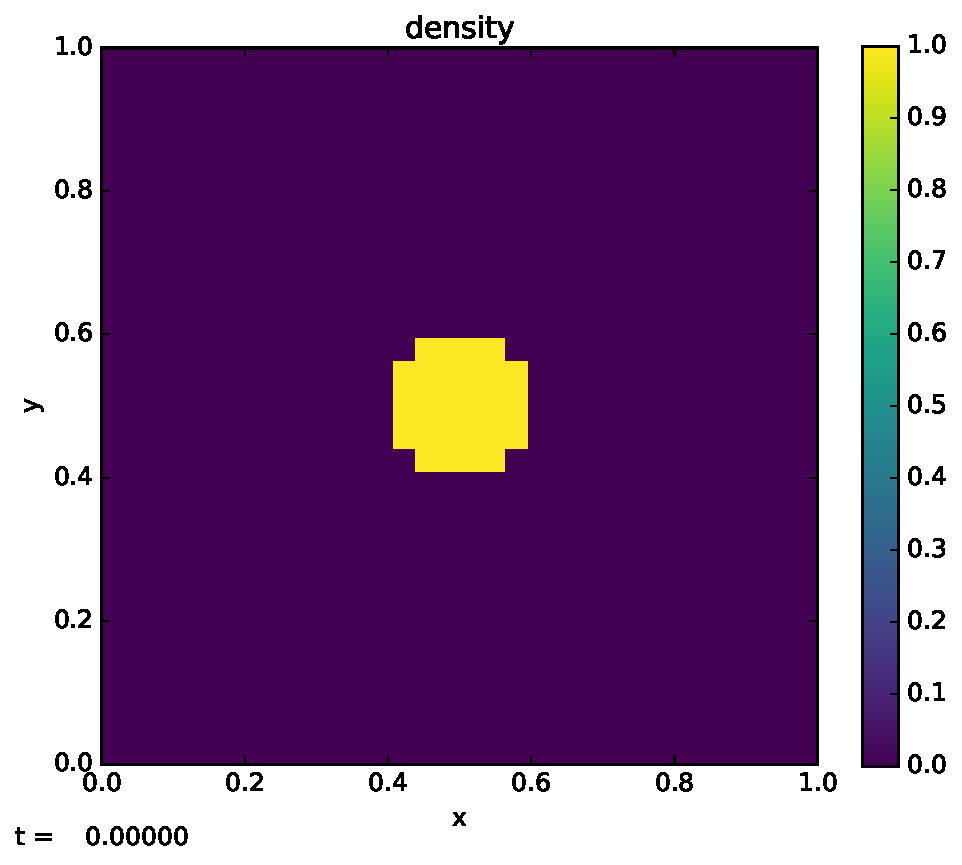
\includegraphics[width=0.48\linewidth]{tophat_init}\hspace{1em}
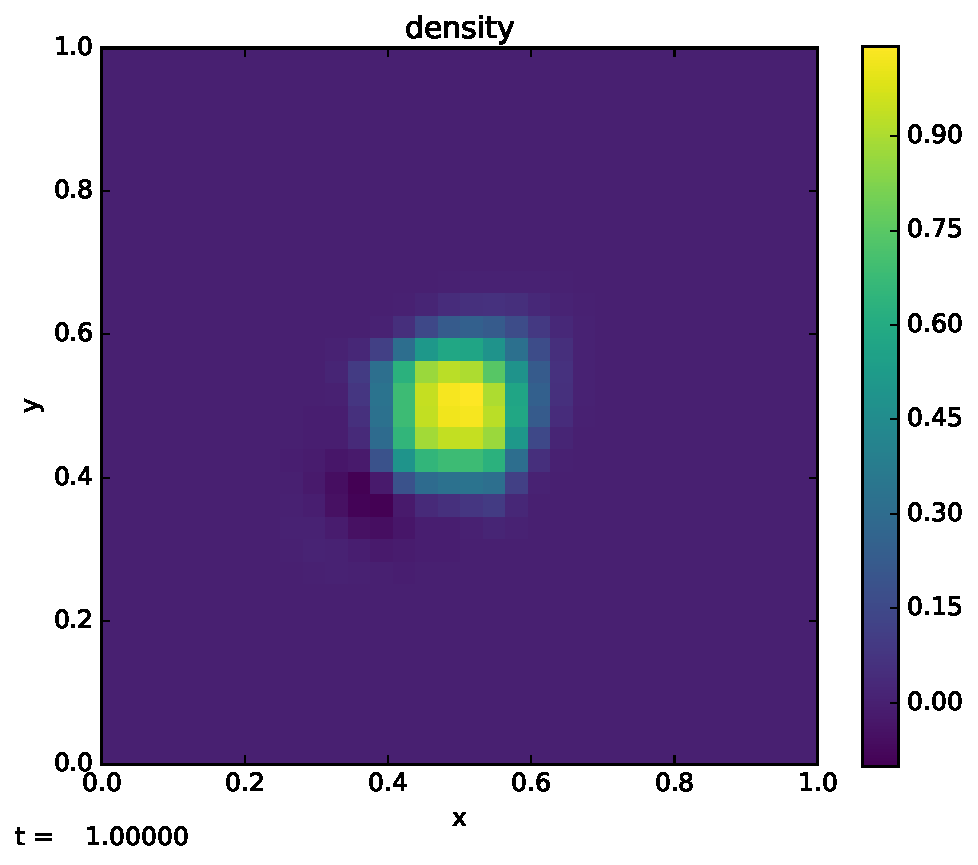
\includegraphics[width=0.48\linewidth]{tophat_final}
\caption[Advection of tophat profile in 2-d]{\label{fig:adv:tophat-2d} Advection of a tophat function with
  $u = v = 1$ for one period on a $32\times 32$ grid, with $\cfl = 0.8$.
  This was run as {\tt ./pyro.py advection tophat inputs.tophat}}
\end{figure}


\subsection{Timestep limiter for multi-dimensions}
\label{sec:adv:timestep}

The timestep criterion we used in one-dimension
(Eq.~\ref{eq:timestep}) needs to be generalized for multi-dimensions.
For the dimensionally split case, since we are basically piecing
together two one-dimensional sweeps, the timestep limit is usually taken
as:
\begin{equation}
\label{eq:adv:timestep:multid}
\Delta t = \cfl \min \left \{ \frac{\Delta x}{|u|} , \frac{\Delta y}{|v|} \right \}
\end{equation}
This is, for example, the construction that is used with the
dimensionally-split hydrodynamics solver in the original Flash
code~\cite{flash}\footnote{although, the paper does not explicitly
  write this out}.  \MarginPar{does the prometheus MPA 449 write it out?}
Stability requires picking a CFL number, $\cfl \le 1$.

A general extension of the timestep restriction for a
fully-multi-dimensional algorithm is often written in the form (see,
e.g., \cite{shuosher:1989b})
\begin{equation}
\label{eq:adv:timstep:mol}
\Delta t = \cfl \left ( \sum_{i=1}^d \frac{|\Ub \cdot \mathbf{e}_d|}{\Delta x_d} \right )^{-1}
\end{equation}
where $d$ is the coordinate direction, $\Ub = (u, v)$ is the velocity
vector, and $\mathbf{e}_d$ is the unit vector in direction $d$.  For
these methods $\cfl \lesssim 1$.  This is usually more restrictive than
Eq.~\ref{eq:adv:timestep:multid}.

For the CTU method described above, \cite{colella:1990} argues that
the inclusion of the transverse information removes some of the some
of the instability inherent in simpler schemes, allowing for a larger
timestep, restricted by Eq.~\ref{eq:adv:timestep:multid}.

Note, because of the different form of the timestep limiters here, it
is not enough to simply cite a CFL number when describing results, you
must also explain which form of the timestep calculation
(Eq.~\ref{eq:adv:timestep:multid} or Eq.~\ref{eq:adv:timstep:mol}) is
being used.

\section{Method of lines approach}
\label{adv:sec:mol_2d}

In the above constructions, we computed a time-centered flux by
predicting the interface state to the half-time (by Taylor-expanding
in time through $\Delta t /2$).  Instead, we can discretize our
equation in space only, giving us an ordinary differential equation
in time that can then be solved using standard ODE techniques.

For example, we can start with Eq.~\ref{eq:adv:multiddivergence}, and define
the fluxes over though a face as:
\begin{itemize}
\item x-face:
\begin{equation}
\langle (ua)_{i+\myhalf,j} \rangle = \frac{1}{\Delta y}
    \int_{y_{j-\myhalf}}^{y_{j+\myhalf}} (ua)_{i+\myhalf,j}\, dy 
\end{equation}
\item y-face
\begin{equation}
\langle (va)_{i,j+\myhalf} \rangle = \frac{1}{\Delta x}
    \int_{x_{i-\myhalf}}^{x_{i+\myhalf}} (va)_{i,j+\myhalf}\, dx 
\end{equation}
\end{itemize}
These are similar to the expressions above, except there is no
integral over time.  Again, to second order in space, we can just
use the flux evaluated at the midpoint in the face:
\begin{equation}
\langle (ua)_{i+\myhalf,j} \rangle \approx (ua)_{i+\myhalf,j}
\end{equation}
The result is the ODE:
\begin{equation}
\frac{d a_{i,j}}{d t} =
   - \frac{(ua)_{i+\myhalf,j} - (ua)_{i-\myhalf,j}}{\Delta x}
   - \frac{(va)_{i,j+\myhalf} - (va)_{i,j-\myhalf}}{\Delta y}
\end{equation}

Note that there is no time-level indicated on the righthand side.  We
find the interface values of $a$ by interpolating in space only, like:
\begin{align}
a_{i+\myhalf,j,L} &= a_{i,j} + \frac{1}{2} \Delta a_{i,j} \\
a_{i+\myhalf,j,R} &= a_{i+1,j} - \frac{1}{2} \Delta a_{i+1,j}
\end{align}
As usual, we resolve the left-right degeneracy on the interface by solving 
the Riemann problem:
\begin{equation}
a_{i+\myhalf,j} = \mathcal{R}(a_{i+\myhalf,j,L}, a_{i+\myhalf,j,R})
\end{equation}
A similar construction is done in the y-direction.  With these
interface states, we have the method for evaluating the righthand side
of our ODE.  We can then evolve the ODE using a Runge-Kutta
integration method.  At each stage of the RK integration, we do the
same construction of the interface states, solve the Riemann problem,
etc.

This construction is a lot simpler than the unsplit method described
previously.  The cost of this simplicity is a reduced range of
stability.  

Performaing the stability analysis here is much more complicated.  For
simplicity, consider a simple first-order upwind scheme in
two-dimensions.  Higher order time integrators (like RK4) will have
separate stages that look like a first-order-in-time update, so this
stability analysis can be thought of as applying to a single stage.
Our difference equation is:
\begin{equation}
\frac{a^{n+1}_{i,j} - a^n_{i,j}}{\Delta t} = - u \frac{a^n_{i,j} - a^n_{i-1,j}}{\Delta x}
- v \frac{a^n_{i,j} - a^n_{i,j-1}}{\Delta y}
\end{equation}
We introduce a single-mode Fourier function, as before, but this time
with a mode in each direction:
\begin{equation}
a^n_{i,j} = A^n e^{Ii\theta}e^{Ij\phi}
\end{equation}
Next, to simplify things, we'll assume that $u = v$, and $\Delta x = \Delta y$, 
then $\cfl = u \Delta t/ \Delta x = v \Delta t / \Delta y$.
Inserting this into our difference equation gives:
\begin{equation}
\frac{A^{n+1}}{A^n} = 1 - \cfl \left (1 - e^{-I\theta} \right ) - \cfl \left (1 - e^{-I\phi} \right )
\end{equation}
This form looks very close to the one-dimensional case, but it is
difficult to analytically find the values of $\cfl$, but we can
numerically find the maximum $ | {A^{n+1}}/{A^n} |^2$ for $\theta \in
[0, 2\pi]$ and $\phi \in [0, 2\pi]$ as a function of $\cfl$.  In doing
this, we find that this discretization is unstable ($| {A^{n+1}}/{A^n}
|^2 > 1$) for $\cfl > 1/2$\footnote{See the script
  \href{https://github.com/zingale/hydro_examples/blob/master/compressible/cfl.py}{cfl.py}}.

This restriction is $1/d$, where $d$ is the dimensionality, and it is
analogous to the difference between the timestep limits for stability
from the more generous Eq.~\ref{eq:adv:timestep:multid} to the more
restrictive Eq.~\ref{eq:adv:timstep:mol}.
This reduced $\cfl$ for stability is discussed in
\cite{shuosher:1989b} (see section 4), and is also discussed in
\cite{titarevtoro,mccorquodalecolella}.  Different reconstruction and
integration methods can vary this limit some, for instance, the fourth-order
method in \cite{mccorquodalecolella} allows for $\Delta t \sum_{i=1}^d (|\Ub \cdot \mathbf{e}_d|)/\Delta x_d  \lesssim 1.4$.  Total variation diminishing Runge-Kutta methods are popular
for this application~\cite{gottliebshu:1996}.

% run as: 
%   ./pyro.py advection_rk tophat inputs.tophat
%   ./plot.py -W 7.7 -H 6 -o tophat_rk4_cfl08.pdf advection_rk tophat_0040
%
%   ./pyro.py advection_rk tophat inputs.tophat driver.cfl=0.4
%   ./plot.py -W 7.7 -H 6 -o tophat_rk4_cfl04.pdf advection_rk tophat_0080
\begin{figure}
\centering
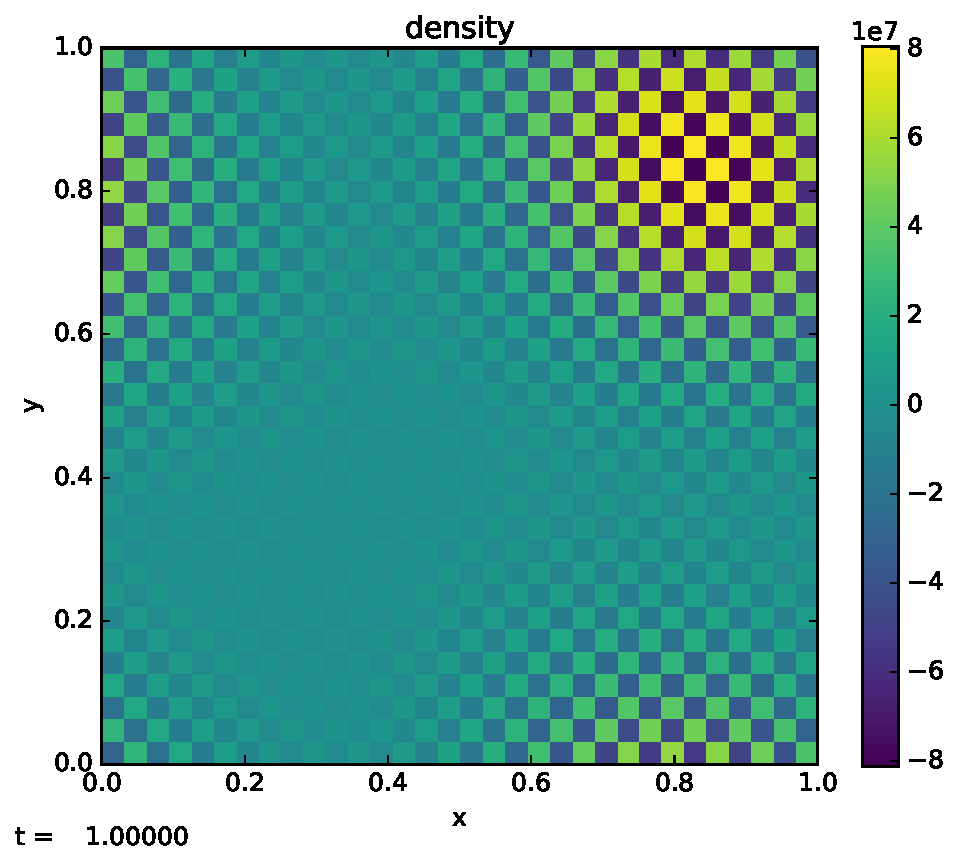
\includegraphics[width=0.48\linewidth]{tophat_rk4_cfl08}\hspace{1em}
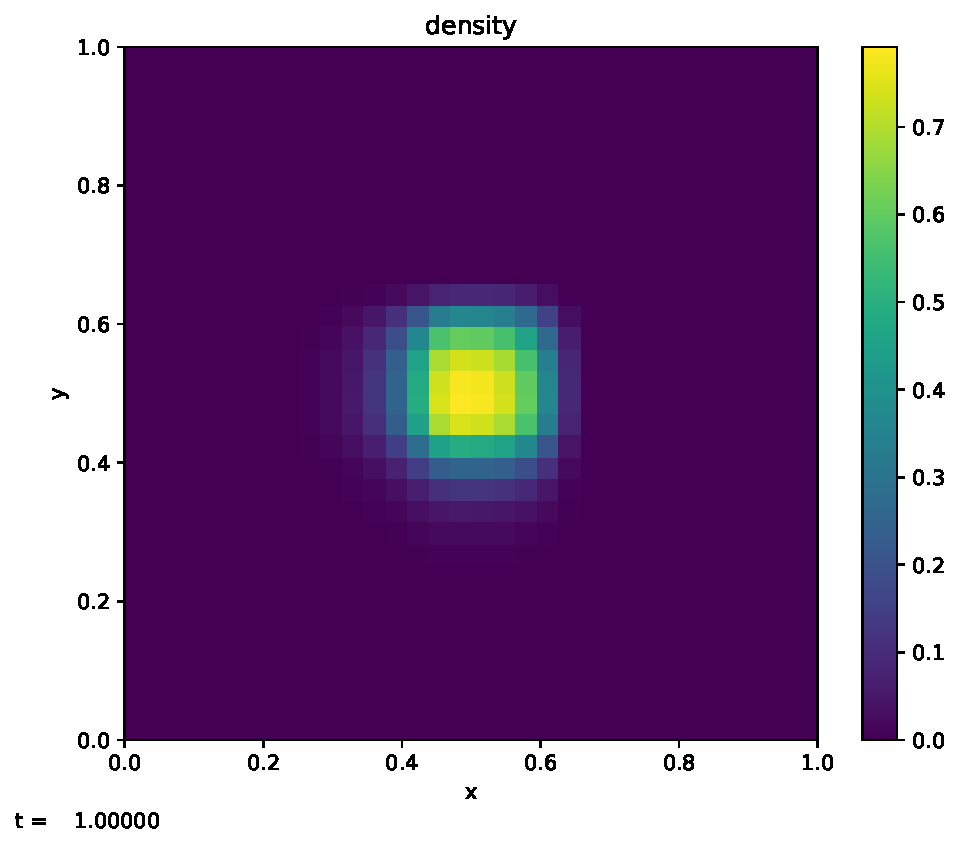
\includegraphics[width=0.48\linewidth]{tophat_rk4_cfl04}
\caption[Advection of tophat function with method-of-lines integration]
  {\label{fig:adv:tophat-2d-rk4} Advection of a tophat function using
  the method-of-lines approach with 4th-order Runge-Kutta time integration.
  We use $u = v = 1$ for one period on a $32\times 32$ grid.  On the left
  is $\cfl = 0.8$---this is clearly unstable.  On the right is $\cfl = 0.4$,
  which is stable.  
  This was run as {\tt ./pyro.py advection\_rk tophat inputs.tophat}}
\end{figure}


\section{Going further}

\begin{itemize}

\item {\em Slope limiting}: there are a wide variety of slope
  limiters.  All of them are designed to reduce oscillations in the
  presence of discontinuities or extrema, but some are higher-order
  and can be less restrictive when dealing with smooth flows.  Most
  hydro texts (e.g.\ \cite{leveque:2002,toro:1997}) provide an
  introduction to the design of such limiters.

\item {\em Multi-dimensional limiting}: the procedure described above
  still does the limiting in each dimension independent of the other
  when doing the unsplit reconstruction.  This can lead to overshoots/
  undershoots.  An example of a method that considers the limiting
  in multi-dimensions is \cite{BDS,quadBDS}.

\item {\em Spatially-varying velocity field}: if we consider a spatially
  varying velocity field, $u(x,y)$ and $v(x,y)$ that is specified externally,
  then we can describe the advection of a quantity $\phi$ as:
  \begin{equation}
  \phi_t + (\phi u)_x + (\phi v)_y = 0
  \end{equation}
  The solution procedure is largely the same as described above.  We write:
\begin{align}
\phi_{i+\myhalf,j,L}^{n+\myhalf} &= \phi_{i,j}^n + 
   \frac{\Delta x}{2} \frac{\partial \phi}{\partial x} +
   \frac{\Delta t}{2} \frac{\partial \phi}{\partial t} + \ldots \nonumber \\
%
 &= \phi_{i,j}^n + 
    \frac{\Delta x}{2} \frac{\partial \phi}{\partial x} +
    \frac{\Delta t}{2} \left [ -(\phi u)_x -(\phi v)_y \right ]_{i,j} \nonumber\\
%
 &= \underbrace{\phi_{i,j}^n + 
   \frac{\Delta x}{2} \left ( 1 - \frac{\Delta t}{\Delta x} u_{i,j} \right )
        \frac{\partial \phi}{\partial x}}_{\hat{\phi}_{i+\myhalf,j,L}^{n+\myhalf}}
   - \frac{\Delta t}{2} \left [\phi u_x \right ]_{i,j} 
   - \frac{\Delta t}{2} \left [ (\phi v)_y \right ]_{i,j}
\end{align}
  and upwinding is used to resolve the Riemann problem for both the
  transverse and normal interface states.  This type of construction
  comes up in low Mach number flows, where the density can be advected
  according to the velocity field in much the fashion shown here, and
  is described in \S~\ref{sec:lm:density}.

  
  For compressible hydrodynamics, we often have density-weighted quantities
  that we advect.  This extension is described in \S~\ref{sec:euler:further}.

\end{itemize}


\section{\pyro\ experimentation}

To gain some experiences with these ideas, we can use the advection 
solver in \pyro\ (see Appendix~\ref{app:pyro} to get started).
The \pyro\ advection solver implements the second-order unsplit
advection algorithm described in the previous sections.  To run
this solver on the Gaussian advection problem, do:
\begin{verbatim}
./pyro.py advection smooth inputs.smooth
\end{verbatim}
By default, this will advect a Gaussian profile diagonally across the
domain for a single period.

To get a feel for the advection algorithm, here are some suggested
exercises:

\begin{exercise}[Role of limiters]
{Implement a tophat initial profile and run with and without limiters
  (this is controlled by the {\tt advection.limiter} runtime
  parameter).}
\end{exercise}

\begin{exercise}[Grid effects]
{Look at the solution when you advect purely in the $x$- or
  $y$-direction and compare to the diagonal case---notice how the
  direction affects the error in the solution.  This is the imprint
  of the grid we discretize on.}
\end{exercise}

\begin{exercise}[Split vs.\ unsplit]
{Implement a dimensionally-split version of the advection algorithm
and compare the results to the unsplit version.  Pick a suitable norm
and measure the convergence of the methods.}
\end{exercise}

